\usepackage{here}
\usepackage{ascmac}
\usepackage{here}
\usepackage{txfonts}
\usepackage{listings, jlisting}
\renewcommand{\lstlistingname}{リスト}
\lstset{
  basicstyle=\ttfamily,
  commentstyle=\textit,
  classoffset=1,
  keywordstyle=\bfseries,
  frame=single,
  framesep=5pt,
  showstringspaces=false,
  numbers=left,
  stepnumber=1,
  numberstyle=\tiny,
  tabsize=2,
  breaklines=true
}

\title{SNS経由で入手される情報のユーザ間差異の可視化}
\author{プロジェクトマネジメントコース\\
ソフトウェア開発管理グループ\\
矢吹研究室\\
1242131\\
吉野 聡志}
\date{}
\begin{document}
\maketitle

\chapter*{謝辞}
本研究において多くのご指導を賜った,矢吹研究室の指導教員である矢吹太朗准教授に厚く御礼申し上げます.また,研究に用いるTwitterタイムラインのデータを提供してくださった矢吹研究室に所属する3年生5人にも,深く感謝の意を表します.

\tableofcontents%目次

\chapter{背景}
世界的に人気のあるSNS(Social Networking Service)のひとつとしてTwitter が存在する.2015年9月30日現在,月間アクティブユーザは3億2000万人である\cite{twitterinc}.

SNSの中でもアクティブユーザ数が非常に多く,利用スタイルも多数あるTwitter に対し,ユーザである人々が顕在的・潜在的に持っているニーズが何であるかが分かれば,他のSNS(Facebook等)との差別化を図りやすくなる.これにより効率的なマーケティングの手法をTwitter社や,Twitter上に広告を打ち出す企業に提案できるのではないか,と考えられる.

\chapter{目的}

\section{目的}
後述する方法で数名のTwitterタイムラインを取得し,各タイムラインで特徴となる単語を抽出する.

第一の目的は,その語群が各人のTwitterにおける関心事項や利用スタイルとどの点が一致するか,またはしないかを見つけることである.

第二の目的は,抽出した単語やTwitterの利用スタイルをユーザごとに比較し,ユーザひとりひとりがどれだけ違った情報をTwitter上でやり取りしているかを見比べることである.

\section{プロジェクトマネジメントとの関連性}
本研究は,情報を「どこから」「どのように」入手し,Twitterユーザのニーズをいかにして読み取るかという手法に着目すると,プロジェクトマネジメント知識エリアの調達マネジメントに属すると考えられる.

\chapter{手法}

\section{本章の構成}
本章では,本研究で利用するTwitterの機能や,研究を行うための環境設定・利用するサービスについて解説したのち,研究の手法について記す.

\section{Twitterとは}
Twitterは,つぶやきと呼ばれる短い発言を投稿し,他のユーザが閲覧・返信することによってコミュニケーションが生まれるSNSである.他のユーザのつぶやきを追跡することを「フォローする」という.タイムラインと呼ばれる画面には,自分のつぶやきとフォローしたユーザのつぶやきが同一画面上に,リアルタイムで表示される.相手がつぶやきを非公開にしていなければ,フォローをする際の承認は不要で,つぶやきを引用することもできる.つぶやきやユーザの検索をすることも可能で,ユーザ同士がつながる機会は多岐にわたる.

\begin{figure}[H]
\centering
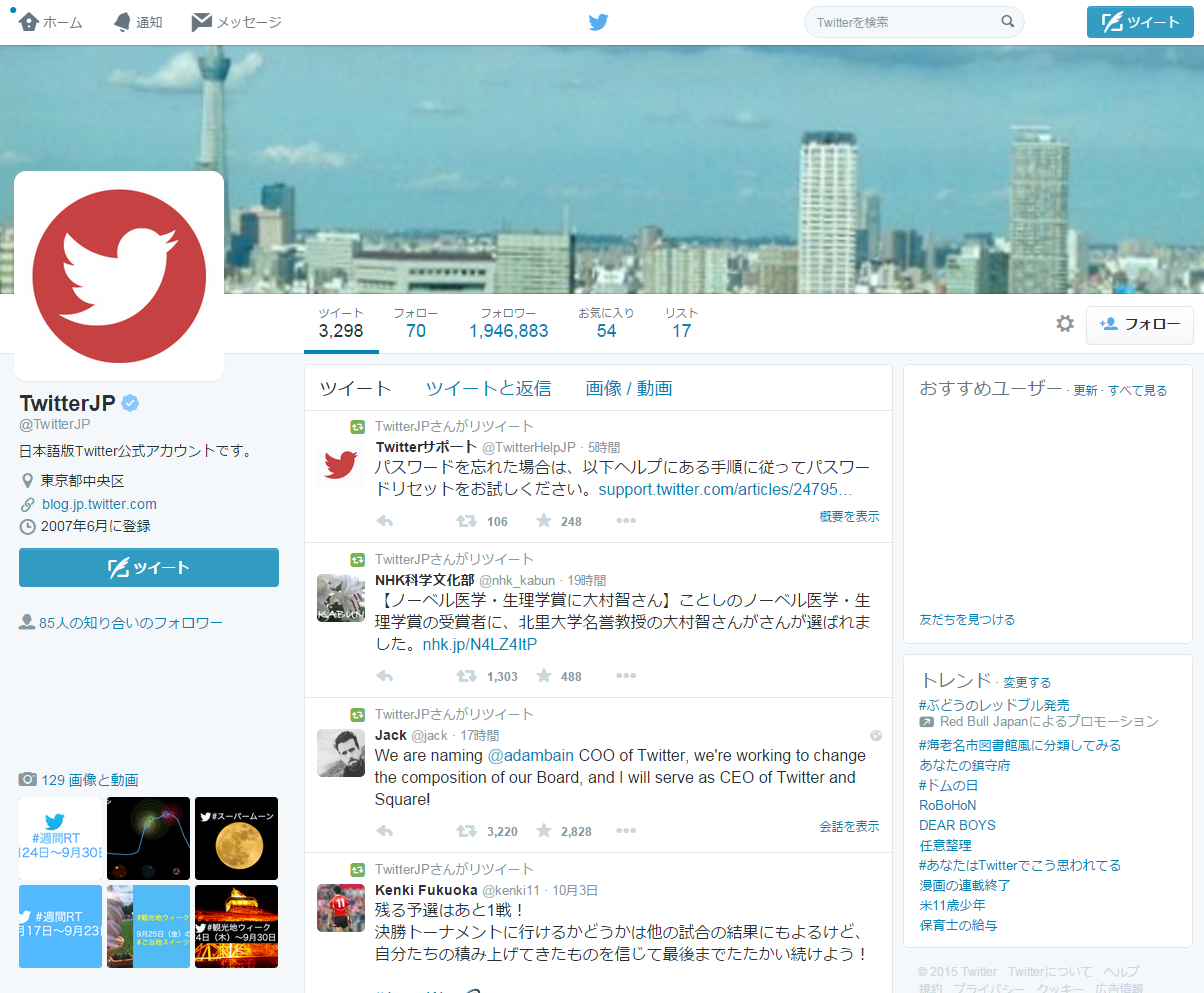
\includegraphics[width=13cm]{TwitterJP.png}
\caption{日本語版Twitter公式アカウントのプロフィールページ}\label{TwitterJP}
\end{figure}

\section{用語}
本節では,本研究で利用するTwitterの用語について説明する\cite{twitterwords}.

\subsection{プロフィールページ}
特定のユーザの自己紹介やつぶやきを表示するページ.Twitterのユーザでない人も閲覧することができる.URLは「https://twitter.com/スクリーンネーム(後述)」となる.

\begin{figure}[H]
\centering
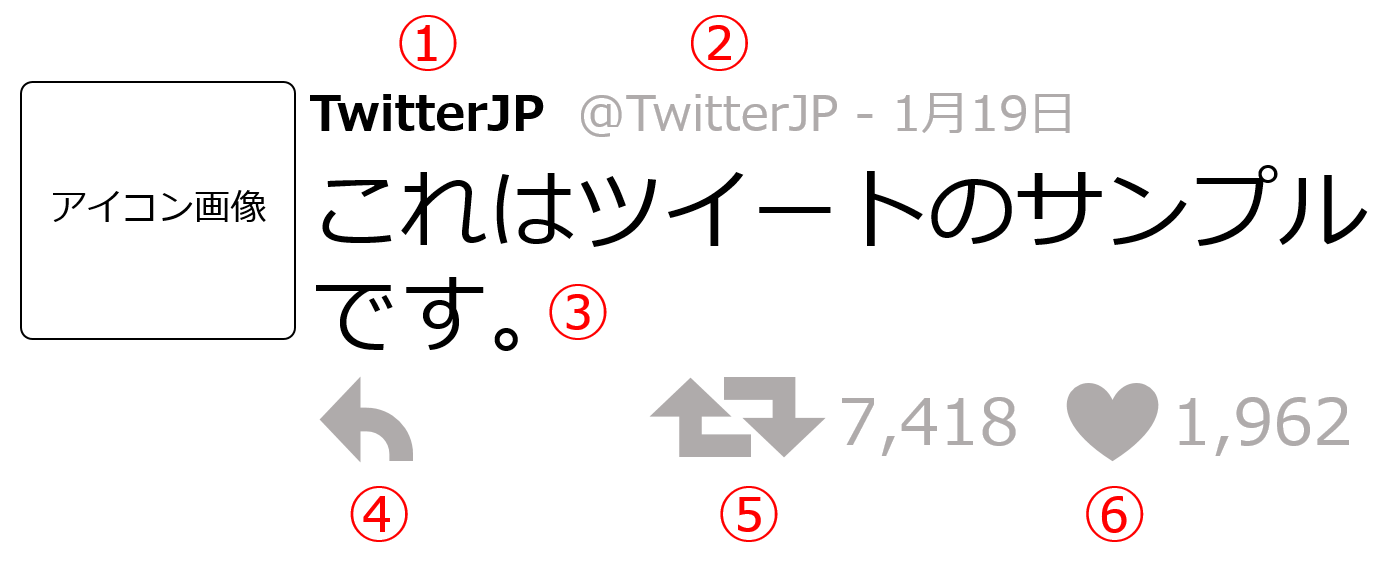
\includegraphics[width=13cm]{tweet_sample.png}
\caption{タイムラインに表示されるツイートの例}\label{tweetsample}
\end{figure}

\subsection{タイムライン}
自分とフォロー(後述)しているユーザのつぶやきがリアルタイムに,時系列に沿って表示される画面.この画面がTwitterでは基本となるため,「ホーム」とも呼ぶ.

\subsection{名前(上図①)}
ユーザのプロフィールページでスクリーンネームとともに表示される名前.後述するスクリーンネームと違い,日本語や記号を入れることができ,他のユーザとの重複があってもそのまま登録できる.登録後のユーザによる変更が可能.

\subsection{スクリーンネーム(上図②)}
ユーザがアカウントを登録する際,ユーザ同士を区別するために設定する名前.最大15文字の半角英数字とアンダースコアの組み合わせからなる.スクリーンネームの先頭には「@」が付く.登録した後,ユーザによる変更が可能.

\subsection{ユーザID}
ユーザがアカウントを登録する際,Twitterがユーザを識別するために決定する数字の羅列.名前やスクリーンネームと異なり,登録した後の変更は不可能.

\subsection{ツイート(上図③)}
Twitterにおける「つぶやき」のこと.1つのツイートにつき160文字まで,という制限が設けられている.ただし,そのうちの20文字はユーザIDに割り当てられているため,残りの140文字がツイートの本文ということになる.

\subsection{リプライ(返信)}
特定のスクリーンネームから始まるツイート.そのユーザ宛のツイートということになる.特定のツイートにリプライする場合,上図④のマークを押す.

\subsection{リツイート}
他のユーザのツイートを,自分のフォロワーに向けてツイートする操作.リツイートをする際は,ツイートの下に表示される上図⑤のマークを押す.自分の手でリツイートしたり,すでに他のユーザによってリツイートされているときは,リツイートされた回数がそのマークの右側に表示される.

\subsection{いいね}
あとで読み返したいと思ったツイートを,自分のいいねリストへ登録する操作.いいねする際は,ツイートの下に表示される上図⑥のマークを押す.リツイートと同じく,いいねされた回数がマークの右側に表示される.

\subsection{フォロー}
特定のユーザのツイートをタイムラインに表示するための操作.

\subsection{フォロワー}
特定のユーザをフォローしているユーザを指す.ユーザAがユーザBをフォローしている場合,ユーザAはユーザBのフォロワーである.

\subsection{位置情報(ジオタグ)}
所在地のデータをツイートに追加し,他のユーザーにどこから投稿しているかを知らせる機能.「位置情報機能」ともいう.

\subsection{メンション}
特定のスクリーンネームを含むツイート.リプライと違い,ツイート内のどこにスクリーンネームが入っていてもメンションとなる.

\subsection{アクティビティ}
自分がフォローしているユーザが他のユーザをフォローしたり,ツイートをお気に入りに登録した等の活動履歴を一覧で表示するページ.フォロー相手の行動をリアルタイムで確認できるため,タイムラインの閲覧だけでは得られない新たな発見の可能性を生み出している.

\subsection{リスト}
ユーザをグループにまとめ,管理する機能.リストごとにタイムラインを表示させることができる.

\subsection{ハッシュタグ}
ツイート内に記載された「\#」から始まる文字列.ハッシュタグを付けてツイートするとその部分が自動的にリンクとなり,クリックすると同じタグが付いたツイートの検索結果が時系列で表示される.

\subsection{トレンド}
Twitter上のツイートの中で多く話題に上っているキーワードをリアルタイムに抽出し,表示する機能.表示するトレンドの地域を設定でき,全世界のトレンドを表示することもできる.

\subsection{ボット(bot)}
Twitterの機能を使って作られた,機械による自動発言システム.ロボット(robot)が語源.特定の時間に自動ツイートするボット,ユーザのボット宛の発言にリプライするボット,特定のキーワードに反応するボット等,様々なボットがある.

\subsection{ダイレクトメッセージ}
送信者と受信者しか見ることができない,非公開のメッセージ.ツイートと違い,1つのメッセージに1万文字まで入力することができる.

\subsection{メール通知}
アカウント作成の際に登録したメールアドレス宛に,自分宛のリプライやダイレクトメッセージの受信をお知らせしてくれる機能.

\subsection{短縮URL}
ツイートの文字数をURL含め140字以内に抑えるため,長いURLを短いURLに変換したもの.代表的なものとしてTwitter公式サービス(http://t.co)がある.

\subsection{非公開ツイート}
フォロワーにのみツイートを公開する設定.非公開ツイートを設定しているユーザのツイートを閲覧するには,その相手に対しフォローリクエストを送信し,許可を得ることが必要となる.

\subsection{認証済みアカウント}
有名人等,多くの人に検索されたり,なりすましの対象になりうるユーザのTwitterアカウントについて,Twitter社が本人確認を行ったアカウント.認証済みアカウントにはプロフィール画面等にチェックマークの入ったブルーの認証バッジが表示される.

\subsection{フォロー解除}
フォローをやめること.リムーブ(remove)とも呼ばれる.

\subsection{ブロック}
特定のユーザからのフォローを取り消し,ブロックされたユーザからのリプライやメンションをブロックした側のアカウントに対して表示させないようにするためのシステム.ブロックしたことがブロックされた側に通知されることはない.ブロックをした,もしくはブロックされたユーザに対しては,ブロックを解除する(される)まではフォローできなくなる.

\subsection{スパム行為}
Twitterにおいてスパム行為とは,不特定多数のユーザに同一内容のツイートやダイレクトメッセージを送り,それらを受け取ったユーザが悪質であると判断したものを指す.ユーザはスパム行為をしていると判断したアカウントをスパムアカウントとして報告することができる.報告が一定数に達するとアカウントが凍結され,そのアカウントのユーザはTwitterを利用できなくなる.ハッシュタグの乱用もスパム行為と見なされ,自動的に凍結されることがある.

\section{Twitter APIについて}
本研究ではTwitterから様々な情報を取得するためのプログラムを使用する.その際に必要となるのがTwitter APIである.本節では,Twitter APIに関する説明をする.

\subsection{API}
アプリケーションプログラムインターフェイス(Application Program Interface)の略で,プログラミングの際に使用できる命令や規約,関数等の集合・枠組みのこと.ソフトウェア開発の際,一からすべてを作るには膨大な時間を要するが,APIという枠組みを利用することにより,プログラミングの負担を軽減することができる\cite{whatsapi}.

\subsection{Twitter API}
Twitter社が提供するAPI.これを利用することでWebサイトやアプリケーションなどからTwitterの機能を呼び出すことができ,ツイートの参照や検索等を行えるアプリケーション開発を行えるようになる\cite{whatstwitterapi}.

\subsection{REST API}
Twitter APIのパラメータ(リソース)を指定し,特定のURLにHTTPでアクセスすると,JSON形式で記述されたメッセージがレスポンスされるシステム.これはツイートの更新や参照を行う際に使用する基本的なAPIとなる.ただし利用制限があり,15分以内に同じ機能を特定の回数利用すると,はじめにその機能を利用した時間から15分経過するまではその機能が利用できなくなる.

\subsection{Streaming API}
今回利用するAPI.タイムラインの変更をリアルタイムに受け取ることができる.REST APIと異なり,利用制限は設けられていない.

\subsection{Access Token}
Twitterに限らず,多くのユーザアカウントに存在するIDとパスワードのような「Access Token」と「Access Token Secret」の2種類の文字列を指す.これは,アプリケーションがユーザの代わりにユーザデータにアクセスするための「通行許可証」のようなものといえる.悪意ある第三者にIDとパスワードそのものを預けた場合,勝手にログインされたり,最悪の場合アカウントを削除することも可能となってしまう.そういったリスクを防ぐため,限られた範囲でユーザデータにアクセスできる権限としてAccess Tokenが利用される\cite{whatsAccessToken}.

\section{Oracle VM VirtualBoxとは}
Oracle VM VirtualBox(以下,VirtualBoxと表記する)は,使用しているPCマシン上に仮想的なマシンを作成し,別のOSをインストール・実行することができるオープンソースソフトウェアである.WindowsやMac OS X,Linux等,様々なOSで利用することができる\cite{VBoxMania}.

\section{用語}
本節では,本研究で利用するVirtualBoxの用語について説明する.

\subsection{ホストマシン(物理マシン)}
物理的に存在するコンピュータ.

\subsection{ホストOS}
ホストマシンにインストールされているOS.VirtualBoxはホストOSにインストールされる.本研究で使用するホストマシンのOSはWindows 7/8.1である. 

\subsection{バーチャルマシン(仮想マシン)}
VirtualBoxが作成する論理的なマシン.VirtualBoxがホストマシンのコンピュータ資源(CPUやメモリ,HDD等)の一部を仮想化し,ゲストマシンに割り当てる.ホストマシンの資源を使いきらない限り,ゲストマシンを複数作成したり,多重起動させることができる.

\subsection{ゲストOS(仮想OS)}
ゲストマシンにインストールされるOS.本研究では,Linuxディストリビューションの一つであるUbuntuをインストールした.

\subsection{仮想ディスク}
ゲストマシンが使用する仮想のハードディスク.バーチャルマシンからはこれを物理ディスクとして扱うことができる.仮想ディスクの実体はホストマシン内にファイルとして存在する.

\subsection{キャプチャ}
Guest Additions(後述)をインストールしていない状態でゲストOSの画面をクリックした際,キーボードやマウスの入力がゲストOSの中でしかできなくなってしまう状態.ホストキー(初期状態では右側のCtrlキー)を押す度に入力先をホストOSとゲストOSに切り替えられるが,その手間を省く等の理由でGuest Additionsをインストールする.

\subsection{Guest Additions}
VirtualBoxの操作性を向上させるためのモジュール.ホストOSとゲストOS間のシームレスなマウスポインタの移動や,ゲストOSの画面の解像度を自由に変更することなどが可能となる\cite{LinuxMania}.これはゲストOSにインストールするため,ゲストマシンごとにインストール作業をする必要がある.

\section{Ubuntuとは}
UbuntuはLinuxのディストリビューション(配布形態)のひとつである.「Ubuntu」という名前はアフリカ・ズールー語で「他者への思いやり」を意味する.その名の通り,使いやすさに重点を置いており,他のディストリビューションと比べて簡単に使い始めることができる\cite{whatsubuntu}.

\subsection{「端末」とは}
Ubuntuをキーボード入力によるコマンドで操作するためのアプリケーション.「ターミナル」とも呼ばれる.Windowsでの「コマンド プロンプト」に相当する.

\section{研究の手法}
本研究では,矢吹研究室に所属する3年生のうち,Twitterのアクティブユーザである5人の協力を得て,各々のマシンやTwitterアカウントを利用してTwitterタイムラインを取得した.所属する研究室の指導教員が自らのブログに記載した方法に則り,Streaming APIを利用してTwitterのタイムラインを取得する.方法は下記のとおりである.

\subsection{VirtualBoxのインストール}
http://www.oracle.com/technetwork/server-storage/virtualbox/downloads/index.htmlをブラウザで開き,「Oracle VM VirtualBox」の項目内から自分の環境に合ったインストーラをダウンロードし,実行する.

\begin{figure}[H]
\centering
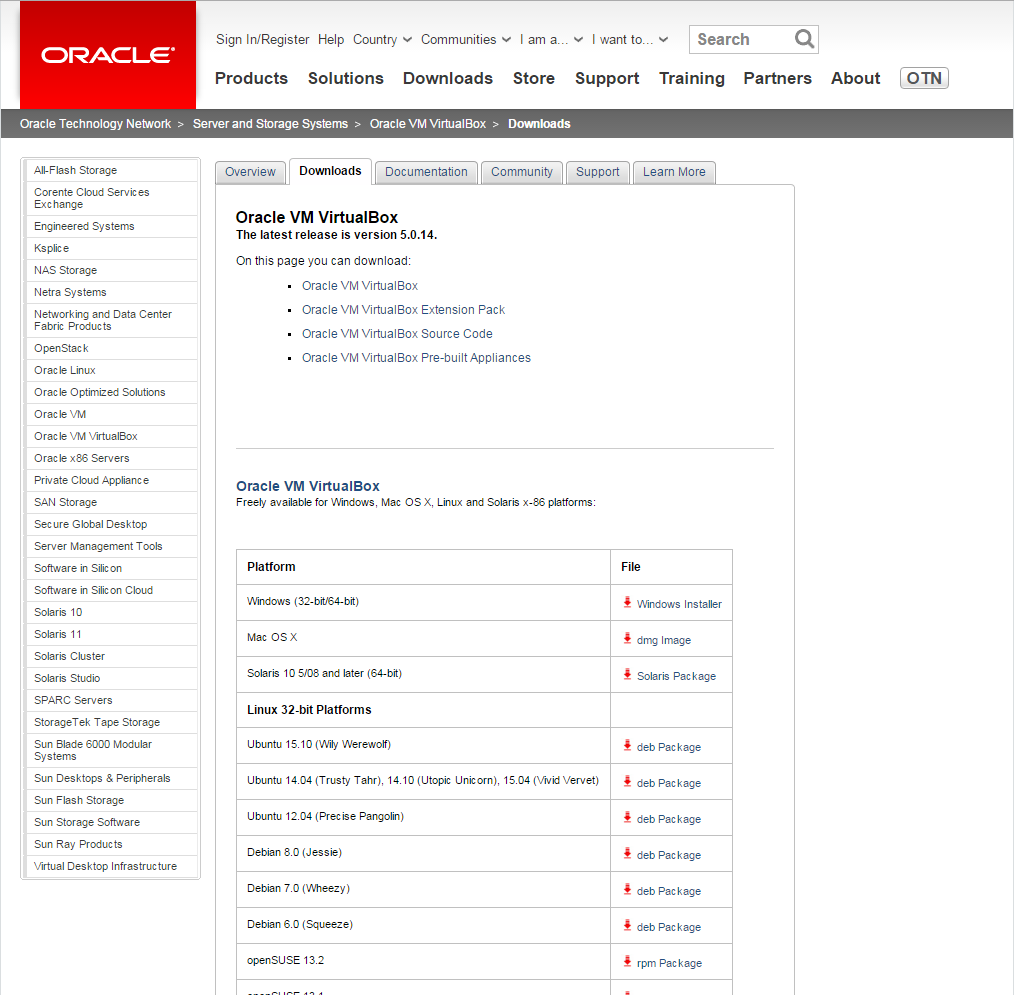
\includegraphics[width=13cm]{virtualboxdownload.PNG}
\caption{http://www.oracle.com/technetwork/server-storage/virtualbox/downloads/index.htmlの表示}\label{vboxdownload}
\end{figure}

インストーラを実行すると以下の画面が表示されるので「Next」を押す.

\begin{figure}[H]
\centering
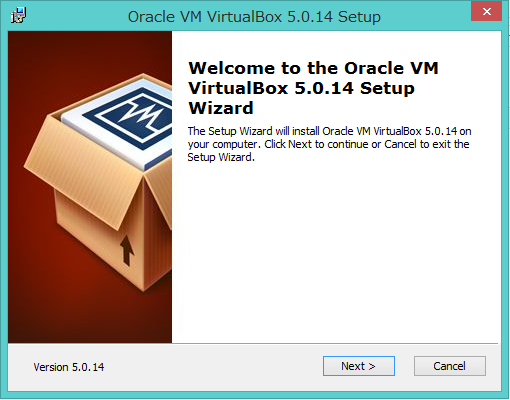
\includegraphics[width=13cm]{vboxinstall_welcome.PNG}
\caption{VirtualBoxセットアップ開始画面}\label{vboxinstallwelcome}
\end{figure}

インストールするコンポーネントの選択をする.特に設定を変更せず,「Next」を押す.

\begin{figure}[H]
\centering
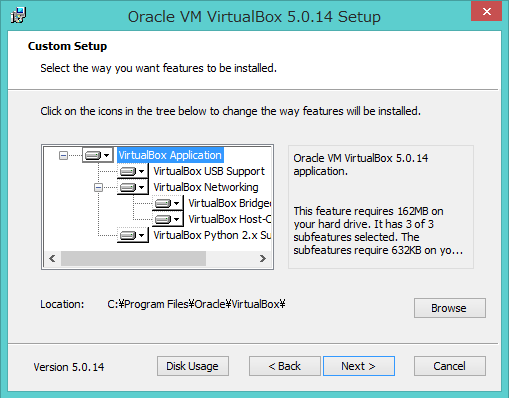
\includegraphics[width=13cm]{vboxinstall_custom.PNG}
\caption{コンポーネント選択画面}\label{vboxinstallcustom}
\end{figure}

インストールオプションを選択し,「Next」を押す.上段からチェックを入れると,

\begin{itemize}
	\item デスクトップ上にアプリケーションのショートカットを作成する
	\item クイック起動にアプリケーションのショートカットを登録する
	\item ファイルの関連付け(拡張子が「.vdi」「.vbox」のもの)を行う
\end{itemize}

という設定になる.

\begin{figure}[H]
\centering
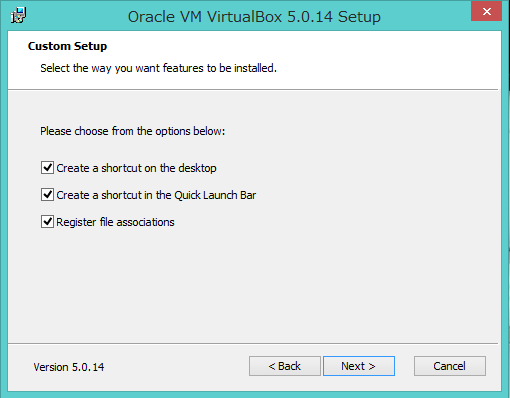
\includegraphics[width=13cm]{vboxinstall_option.PNG}
\caption{インストールオプション選択画面}\label{vboxinstalloption}
\end{figure}

ネットワークインターフェイスに関する警告が出るので,「Yes」を押す.

\begin{figure}[H]
\centering
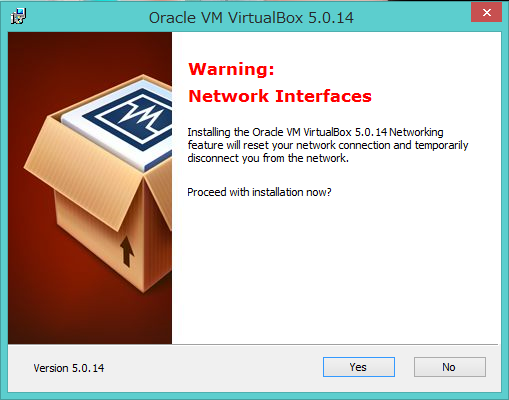
\includegraphics[width=13cm]{vboxinstall_network.PNG}
\caption{ネットワークインターフェイスに関する警告画面}\label{vboxinstallnetwork}
\end{figure}

この画面が表示されるとインストールの準備が完了する.「Install」を押すとインストールが開始される.

\begin{figure}[H]
\centering
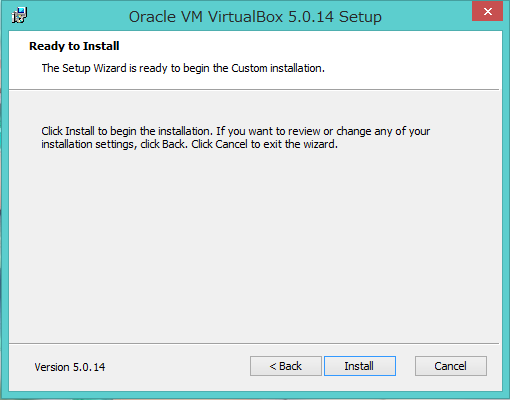
\includegraphics[width=13cm]{vboxinstall_ready.PNG}
\caption{インストール準備完了画面}\label{vboxinstallready}
\end{figure}

使用するPCの設定によっては,ユーザー アカウント制御の画面が表示され,インストールの許可をするかどうか尋ねてくる.その場合は,「はい(Y)」を押して続行する.

\begin{figure}[H]
\centering
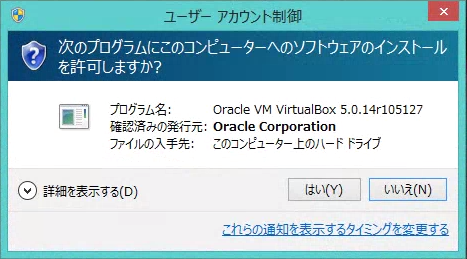
\includegraphics[width=13cm]{vboxinstall_uac.PNG}
\caption{ユーザー アカウント制御画面}\label{vboxinstalluac}
\end{figure}

VirtualBoxで利用するUSBコントローラーをインストールするかどうか尋ねてくるので,「インストール(I)」を押す.

\begin{figure}[H]
\centering
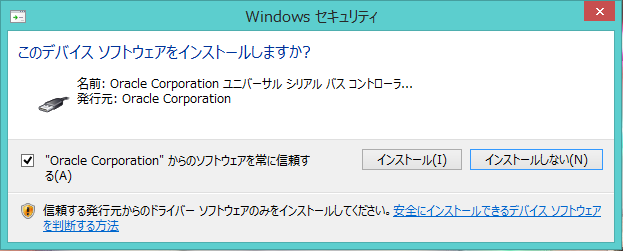
\includegraphics[width=13cm]{vboxinstall_device.PNG}
\caption{USBコントローラーをインストールするか尋ねる画面}\label{vboxinstalldevice}
\end{figure}

インストールが完了すると以下の画面が表示される.チェックを入れた状態で「Finish」を押すとVirtualBoxが起動する.

\begin{figure}[H]
\centering
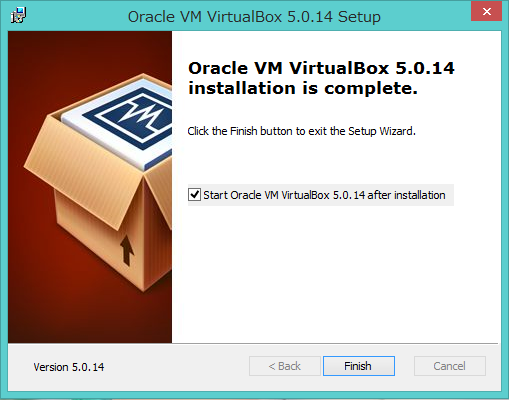
\includegraphics[width=13cm]{vboxinstall_finish.PNG}
\caption{インストール完了画面}\label{vboxinstallfinish}
\end{figure}

\subsection{Ubuntuのインストール}
まず,https://www.ubuntulinux.jp/download/ja-remixよりUbuntu 14.04のISOイメージをダウンロードする.本研究では64bit版を選択した.

\begin{figure}[H]
\centering
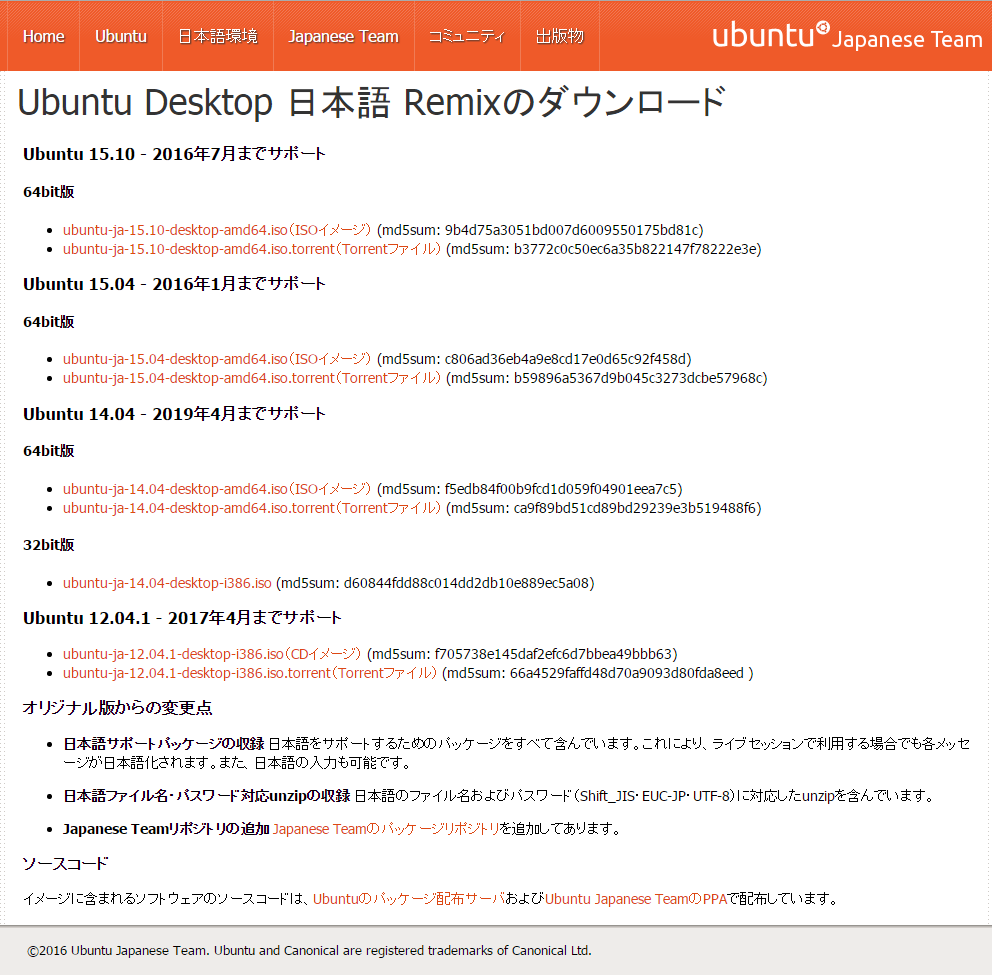
\includegraphics[width=13cm]{ubuntudownload.PNG}
\caption{https://www.ubuntulinux.jp/download/ja-remixの表示}\label{ubuntudownload}
\end{figure}

次にインストールしたVirtualBoxを立ち上げ,ウィンドウ左上にある「新規(N)」のボタンを押してゲストマシンの作成を行う.ゲストマシンの名前,メモリサイズ,HDDの設定をするとウィンドウが閉じられる.
	
\begin{figure}[H]
\centering
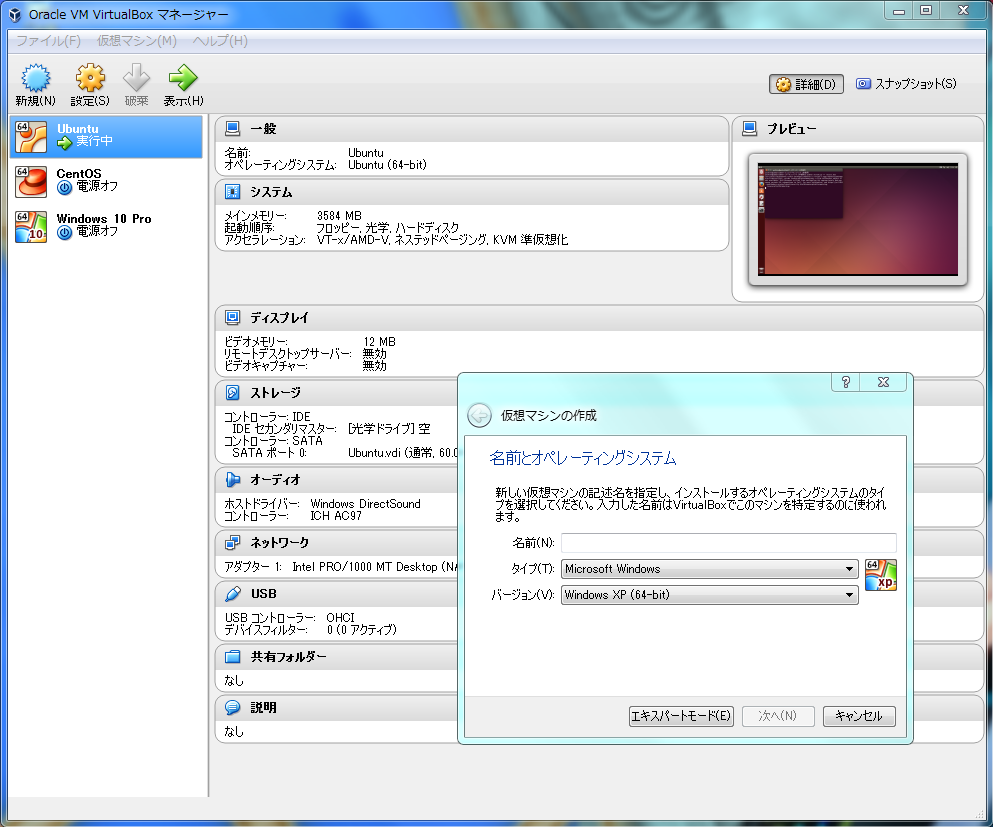
\includegraphics[width=13cm]{VBoxWindow.PNG}
\caption{VirtualBoxのウィンドウとゲストマシン作成ウィンドウ}\label{VBoxSetup}
\end{figure}

HDDの設定は以下のように行う.まず,「仮想ハードディスクを作成する(C)」を選択して「作成」を押す.

\begin{figure}[H]
\centering
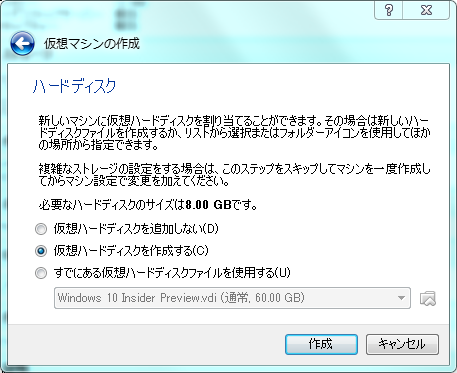
\includegraphics[width=13cm]{vdi_create.PNG}
\caption{仮想HDD作成画面}\label{vdicreate}
\end{figure}

VDI(VirtualBox Disk Image)を選択して「次へ(N)」を押す.

\begin{figure}[H]
\centering
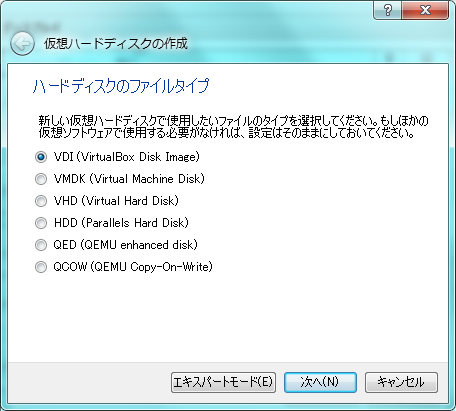
\includegraphics[width=13cm]{vdi_type.PNG}
\caption{HDDのファイルタイプ選択画面}\label{vditype}
\end{figure}

固定サイズ(F)を選択して「次へ(N)」を押す.

\begin{figure}[H]
\centering
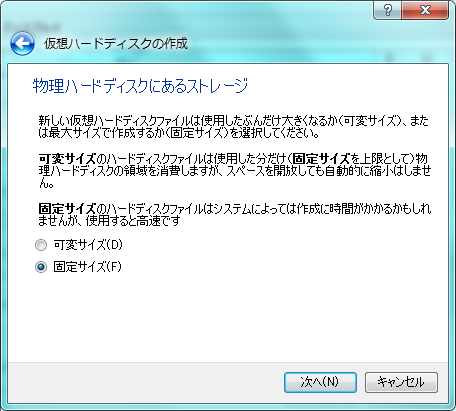
\includegraphics[width=13cm]{vdi_size_kotei.PNG}
\caption{仮想HDDのサイズタイプ選択画面}\label{vdisizekotei}
\end{figure}

HDDのサイズを設定し,「作成」を押す.本研究では60GBに設定した.

\begin{figure}[H]
\centering
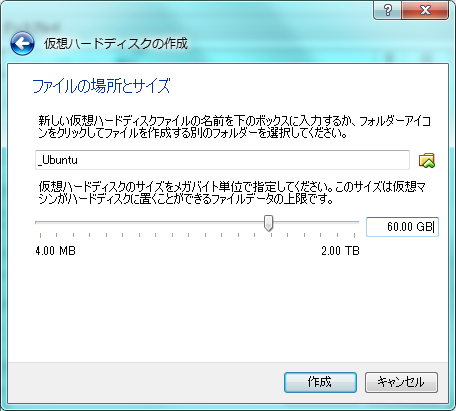
\includegraphics[width=13cm]{vdi_size.PNG}
\caption{仮想HDDサイズ設定画面}\label{vdisize}
\end{figure}

仮想HDDの作成中,以下の画面が表示される.完了すると自動でこの画面は閉じられる.

\begin{figure}[H]
\centering
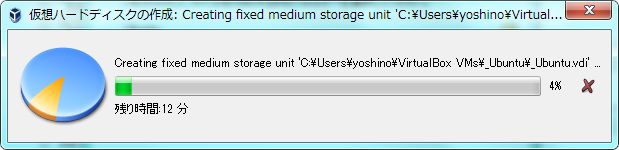
\includegraphics[width=13cm]{vdi_creating.PNG}
\caption{仮想HDD作成中画面}\label{vdicreating}
\end{figure}

続いて「設定(S)」を開き,「ストレージ」の項目にあるストレージツリーより,「コントローラー: IDE」内の「空」を選択する.「属性」内にあるディスクのマークをクリックしてプルダウンメニューを開き,「仮想光学ディスクファイルを選択...」をクリックしてダウンロードしたISOイメージをマウントする.
	
\begin{figure}[H]
\centering
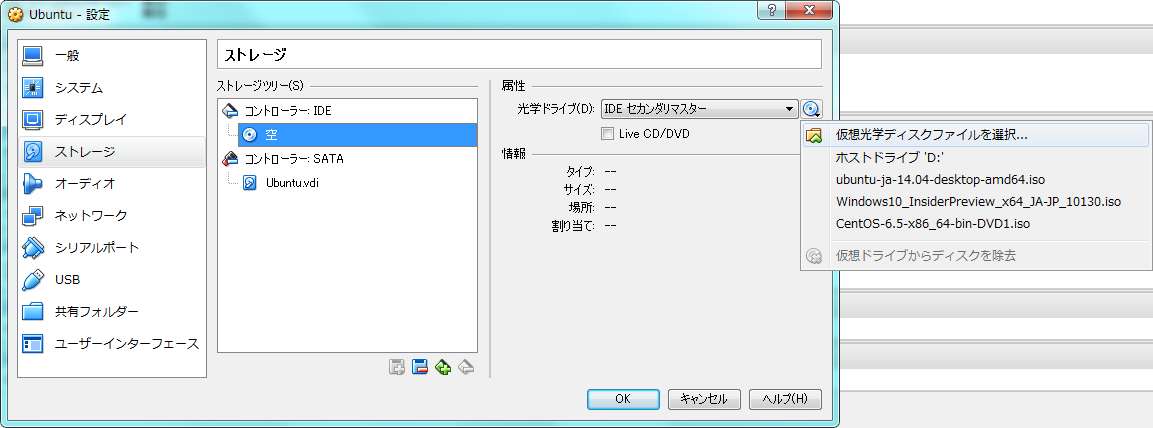
\includegraphics[width=13cm]{iso_set.png}
\caption{ISOイメージのマウント}\label{isoset}
\end{figure}
	
「OK」をクリックして「起動(T)」を押すとゲストマシンが起動し,Ubuntuのインストールウィザードが表示されるので,「Ubuntuをインストール」を押す.
	
\begin{figure}[H]
\centering
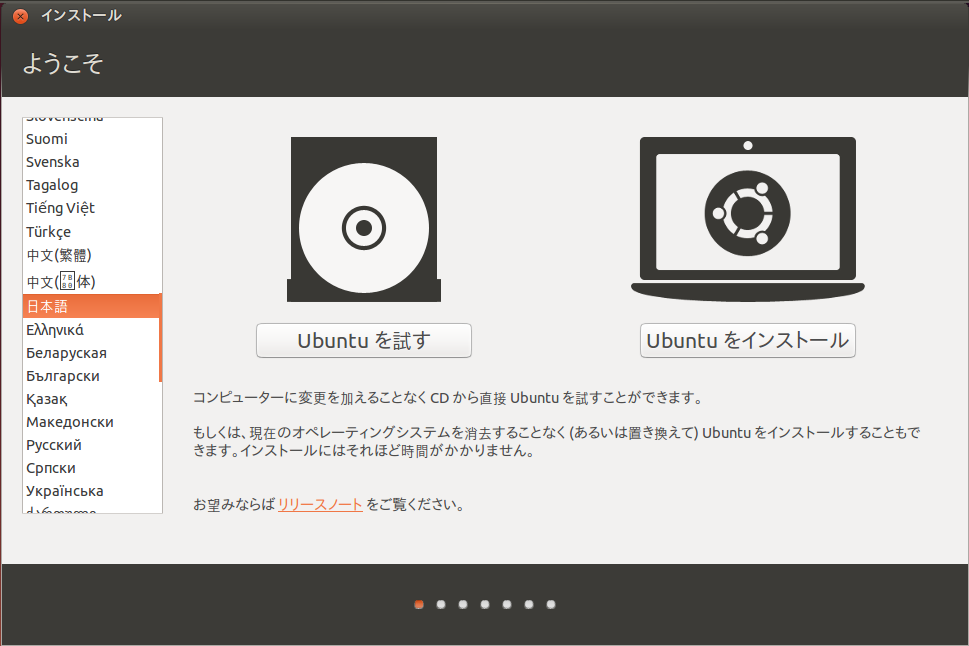
\includegraphics[width=13cm]{ubuntuinstall01.PNG}
\caption{「ようこそ」画面}\label{ubuntuinstall01}
\end{figure}
	
「インストール中にアップデートをダウンロードする」のチェックボックスにチェックを入れ,「続ける」をクリックする.
	
\begin{figure}[H]
\centering
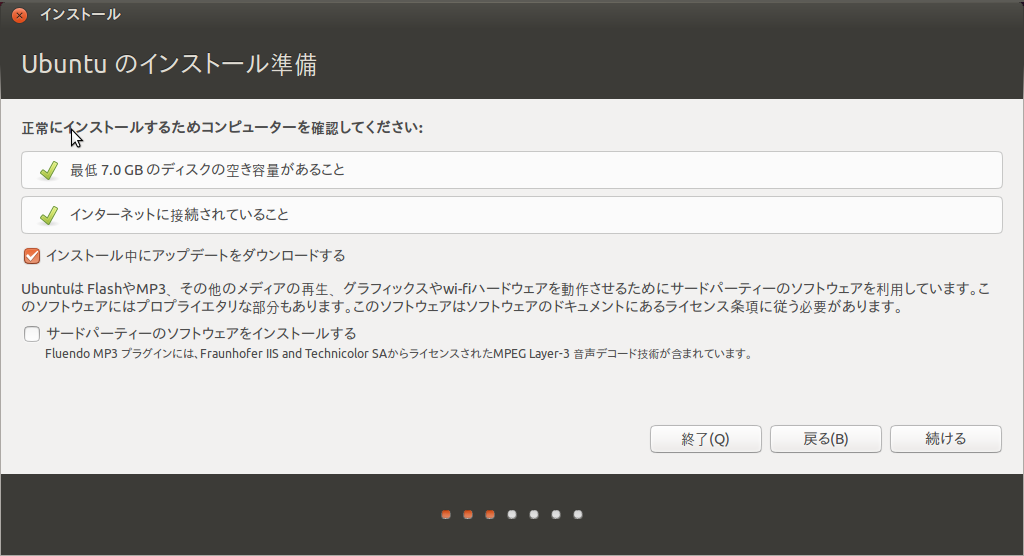
\includegraphics[width=13cm]{ubuntuinstall02.PNG}
\caption{「Ubuntuのインストール準備」画面}\label{ubuntuinstall02}
\end{figure}
	
「ディスクを削除してUbuntuをインストール」のラジオボタンを選択し,インストール(I)をクリックする.
	
\begin{figure}[H]
\centering
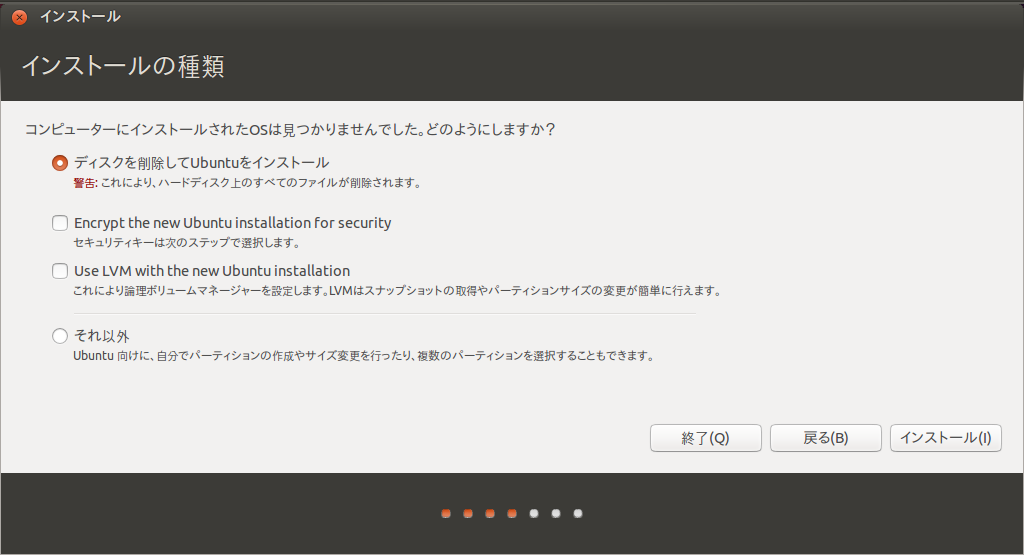
\includegraphics[width=13cm]{ubuntuinstall03.PNG}
\caption{「インストールの種類」画面}\label{ubuntuinstall03}
\end{figure}
	
居住地の入力を行い,「続ける」をクリックする.デフォルトの「Tokyo」のまま進めても問題はない.
	
\begin{figure}[H]
\centering
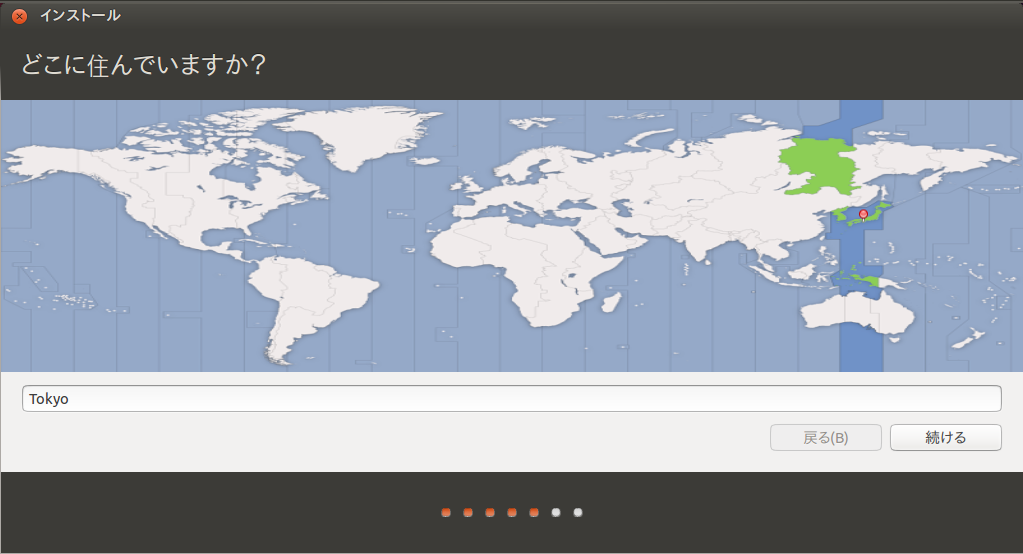
\includegraphics[width=13cm]{ubuntuinstall04.PNG}
\caption{「どこに住んでいますか?」画面}\label{ubuntuinstall04}
\end{figure}

キーボードレイアウトの選択を求められる.左右ともに「日本語」になっていることを確認し,「続ける」をクリックする.

\begin{figure}[H]
\centering
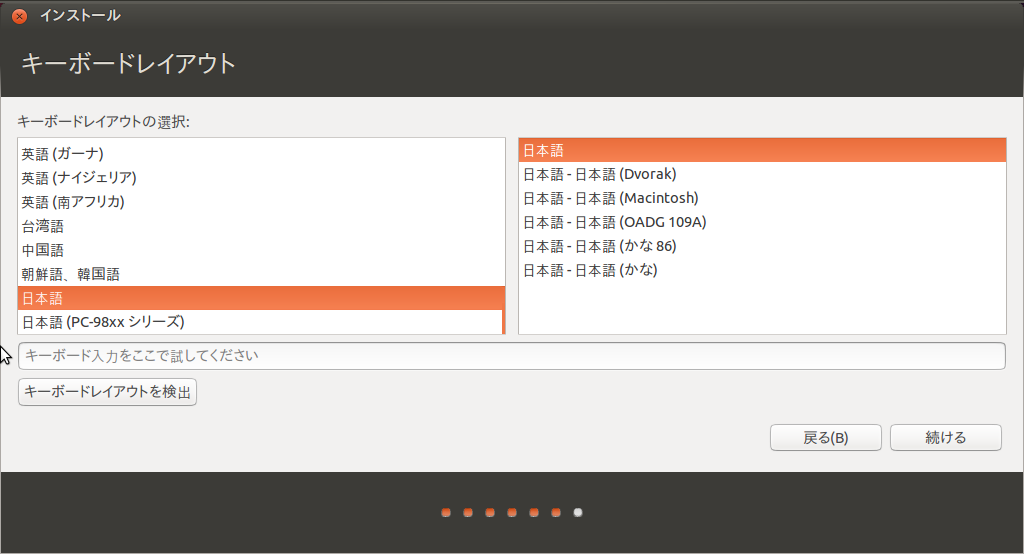
\includegraphics[width=13cm]{ubuntuinstall05.PNG}
\caption{「キーボードレイアウト」画面}\label{ubuntuinstall05}
\end{figure}

各テキストボックスに情報を入力し,「続ける」をクリックするとインストールが開始される.

\begin{figure}[H]
\centering
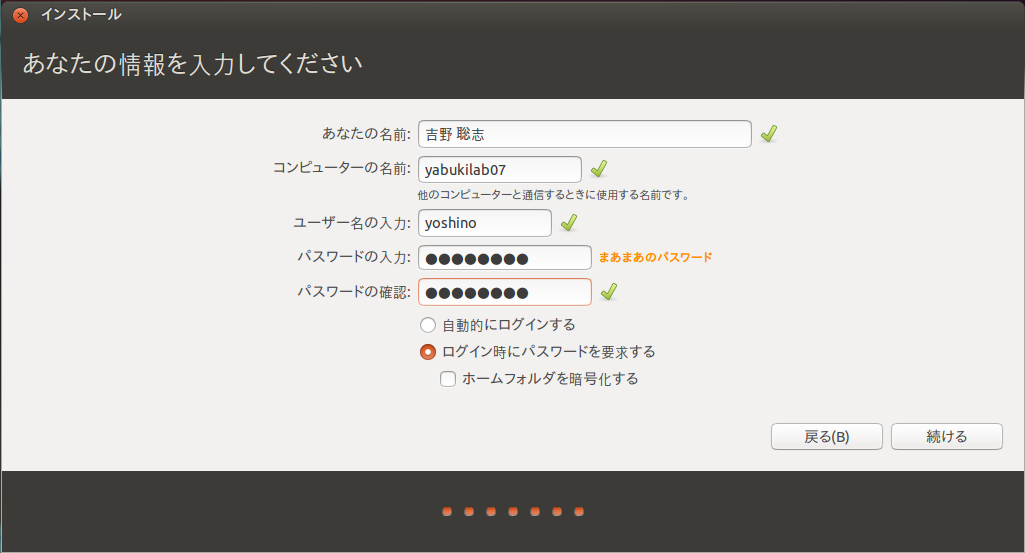
\includegraphics[width=13cm]{ubuntuinstall06.PNG}
\caption{「あなたの情報を入力してください」画面}\label{ubuntuinstall06}
\end{figure}

インストールが完了すると再起動を求められるので,「今すぐ再起動する」をクリックする.

\begin{figure}[H]
\centering
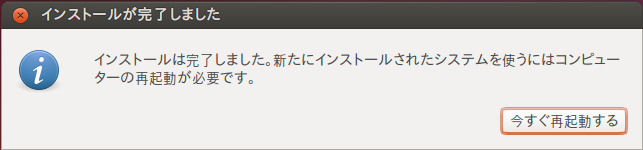
\includegraphics[width=13cm]{ubuntuinstallfinished.PNG}
\caption{「インストールが完了しました」ウィンドウの表示}\label{ubuntuinstallfinished}
\end{figure}

この画面になり,青い文字で「Please remove installation media and close the tray (if any) ten press ENTER:」と表示されたらEnterキーを押して再起動する.

\begin{figure}[H]
\centering
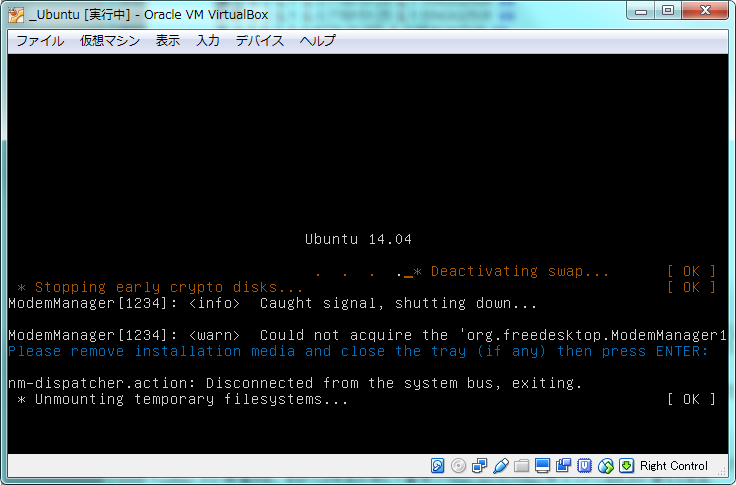
\includegraphics[width=13cm]{press_enter.PNG}
\caption{Enterキーの入力を求める画面}\label{pressenter}
\end{figure}

\subsection{Guest Additionsのインストール}
ゲストマシンにインストールしたUbuntuを立ち上げ,ホストOS側のメニューバーにある「デバイス」から「Guest Additions CD イメージの挿入...」を選択するとウィンドウが開く.

\begin{figure}[H]
\centering
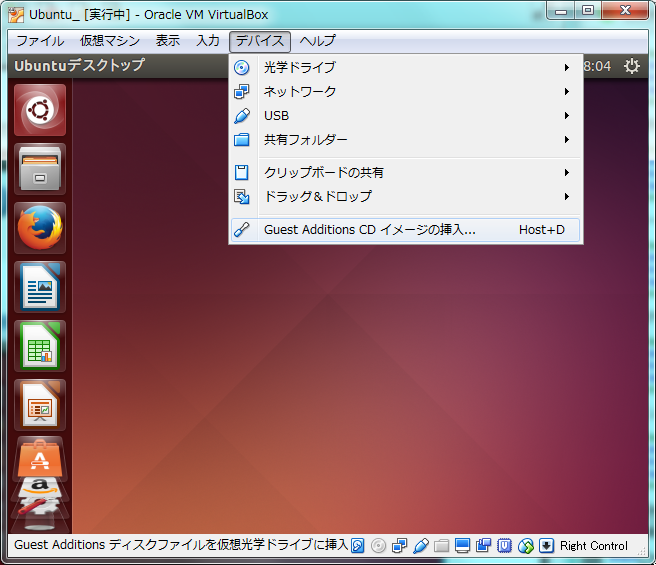
\includegraphics[width=13cm]{ubuntuguestadditionsinstall01.PNG}
\caption{Guest Additions CD イメージの挿入}\label{ubuntuguestadditionsinstall01}
\end{figure}
	
「実行する(R)」を押すとパスワードの入力を求められるので,Ubuntuインストール時に登録したパスワードを入力し,認証する(A)をクリックしてインストールを開始する.

\begin{figure}[H]
\centering
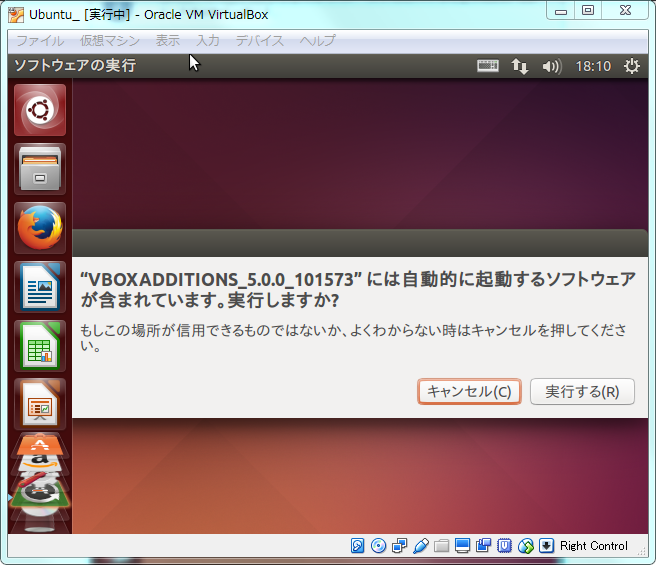
\includegraphics[width=13cm]{ubuntuguestadditionsinstall02.PNG}
\caption{「ソフトウェアの実行」画面}\label{ubuntuguestadditionsinstall02}
\end{figure}
	
\begin{figure}[H]
\centering
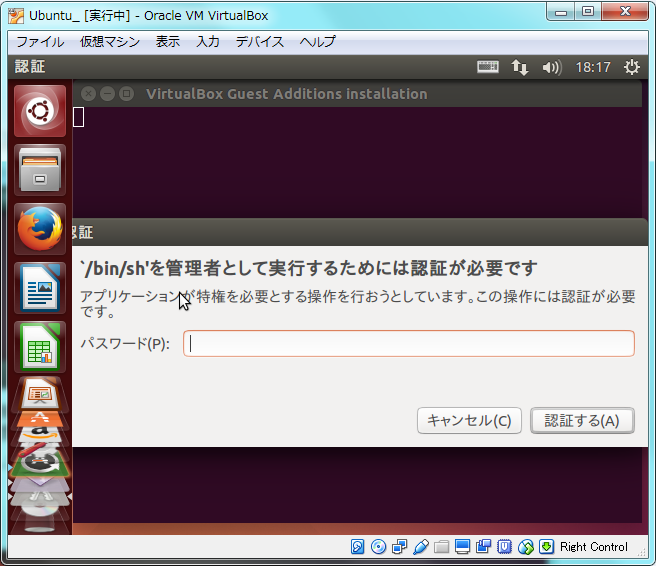
\includegraphics[width=13cm]{ubuntuguestadditionsinstall03.PNG}
\caption{パスワード入力画面}\label{ubuntuguestadditionsinstall03}
\end{figure}
	
「Press Return to close this window...」と表示され,Enterキーを押すとインストールが完了する.

\begin{figure}[H]
\centering
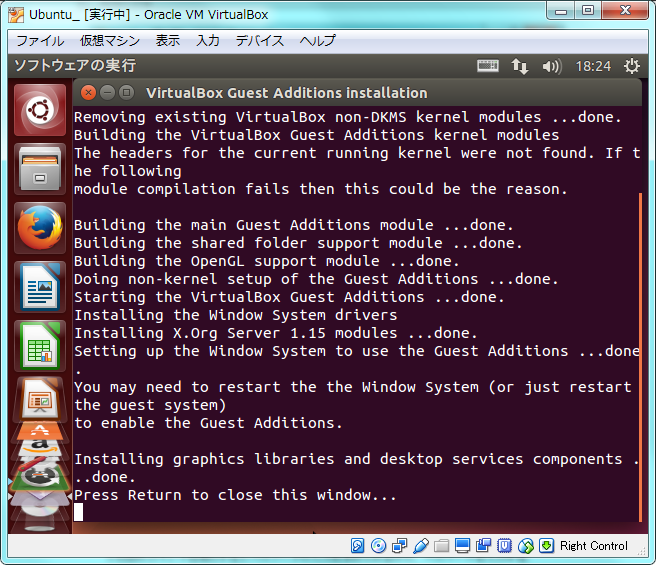
\includegraphics[width=13cm]{ubuntuguestadditionsinstallfinished.PNG}
\caption{インストール完了画面}\label{ubuntuguestadditionsinstallfinished}
\end{figure}

画面右上にある電源マークを押してプルダウンメニューを表示させ,「シャットダウン...」を押す.

\begin{figure}[H]
\centering
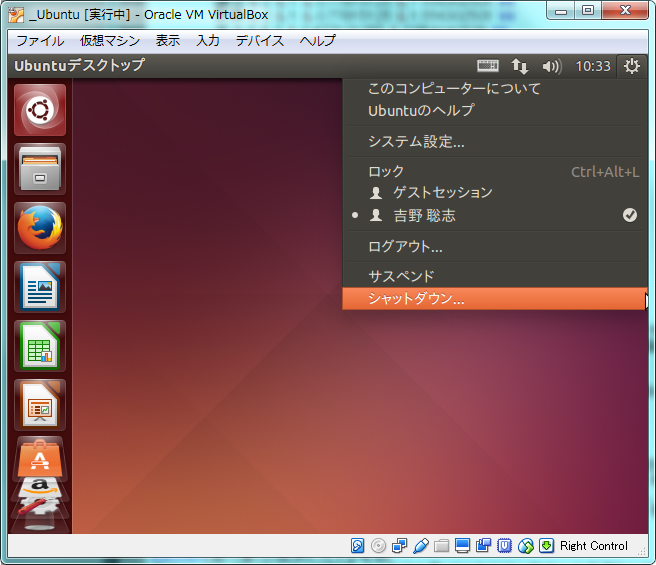
\includegraphics[width=13cm]{ubuntushutdown.PNG}
\caption{プルダウンメニュー表示画面}\label{ubuntushutdown}
\end{figure}

左側のボタンを押して仮想マシンを再起動させるか,右側のボタンを押してシャットダウンさせるとGuest Additionsのインストールが完了する.

\begin{figure}[H]
\centering
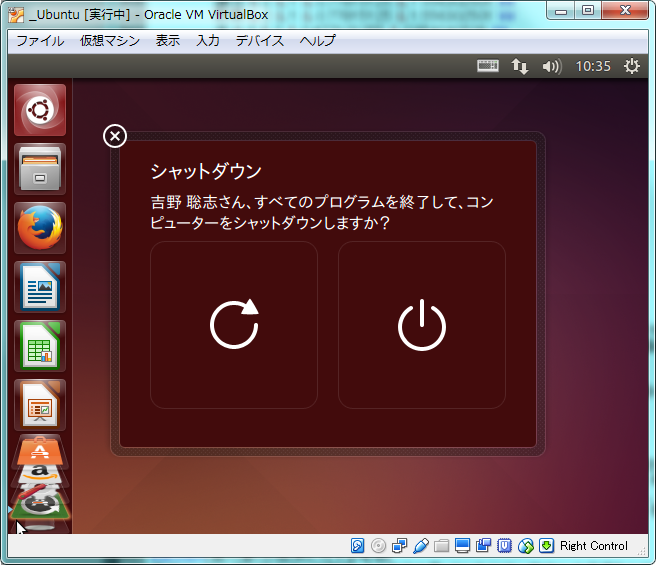
\includegraphics[width=13cm]{ubuntushutdown_choose.PNG}
\caption{再起動するかシャットダウンするかを選択する画面}\label{ubuntushutdownchoose}
\end{figure}

\subsection{Tweepyのインストール}
Tweepyとは,プログラム言語PythonでTwitterを利用するためのライブラリである.以下にTweepyのインストール手順を記す.
Ubuntuでは,アプリケーションを素早く起動するボタンを設置したり,実行中のタスク一覧を表示するLauncherがデスクトップ左側に表示される.その最上部にあるUbuntuのロゴを押すと,バーチャルマシン内に存在するファイルやアプリケーション等を検索できるウィンドウが表示される.

\begin{figure}[H]
\centering
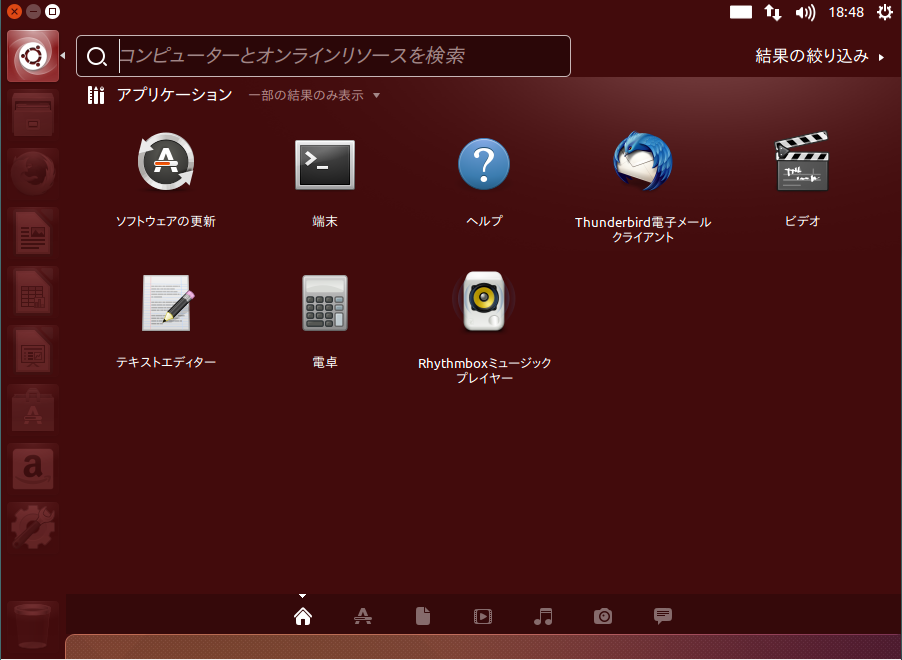
\includegraphics[width=13cm]{super1.PNG}
\caption{検索画面の表示}\label{super1}
\end{figure}

ウィンドウ下部に並ぶアイコンのうち,左から2つ目のものを押すとアプリケーションの検索画面に遷移する.その画面内にある「インストール済み」を押すと,インストールされたアプリケーションの一覧が表示されるので,その中より「端末」を起動させる.

\begin{figure}[H]
\centering
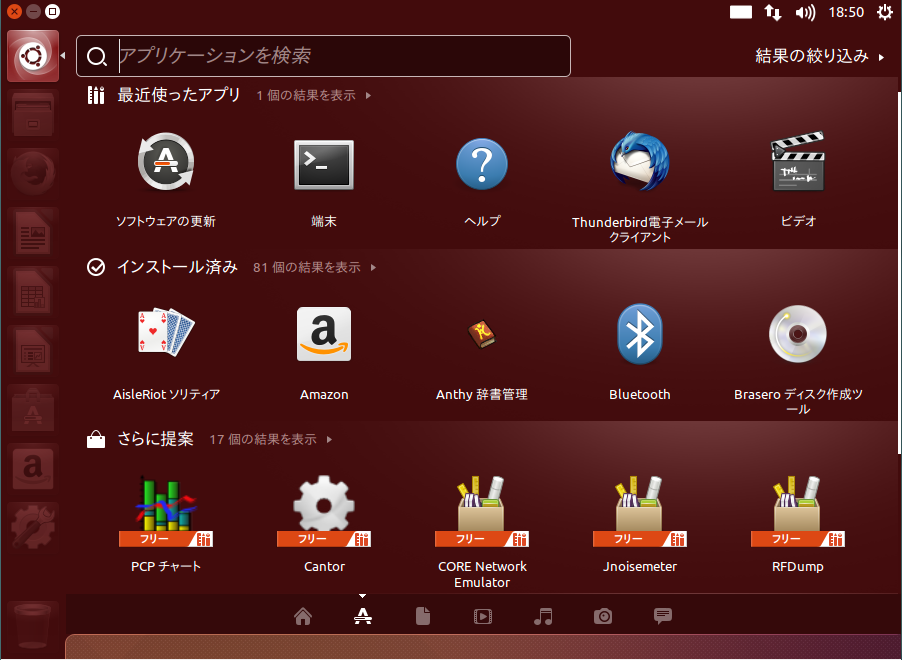
\includegraphics[width=13cm]{super2.PNG}
\caption{インストールされているアプリケーション一覧の表示}\label{super2}
\end{figure}

\begin{figure}[H]
\centering
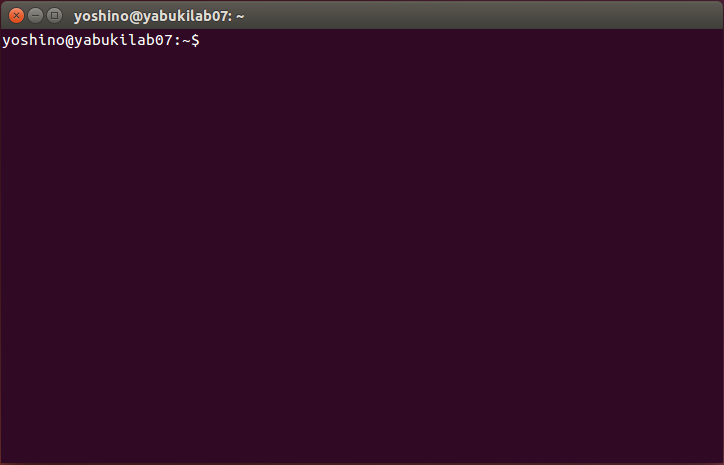
\includegraphics[width=13cm]{terminal.PNG}
\caption{「端末」ウィンドウ}\label{terminal}
\end{figure}

1行目のコマンドを実行するとパスワードの入力を求められるので,パスワードを入力する.パスワードを入力しても画面には反映されないが,無視して入力し,Enterキーを押すとPythonのインストールが開始される.
	
\begin{lstlisting}[caption={}, label={}]
	sudo apt-get install python-setuptools python-pip
	sudo easy_install tweepy
\end{lstlisting}
	
途中,続行するかどうかを尋ねられるので,「y」を入力し,Enterを押す.
	
\begin{figure}[H]
\centering
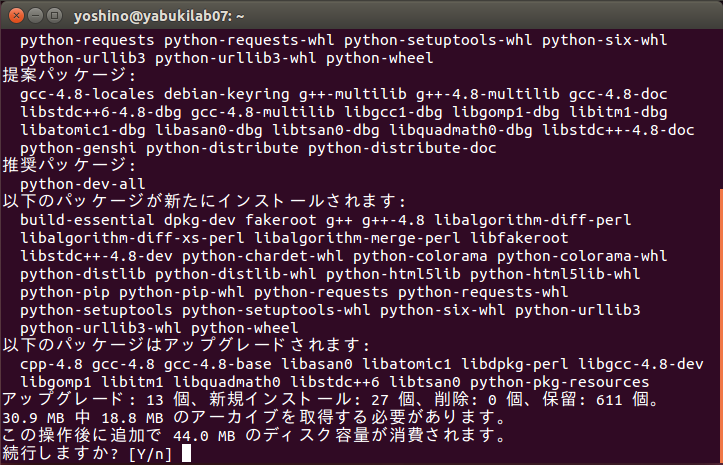
\includegraphics[width=13cm]{pythoninstall.PNG}
\caption{続行するかどうかを尋ねる表示}\label{pythoninstall}
\end{figure}

インストールが完了したら,続けて2行目のコマンドを入力し,Tweepyのインストールを実行する.
	
\subsection{Twitterでの携帯電話番号を用いた認証}
Twitter APIを利用するにはまず,自らが持つ携帯電話の番号をTwitter上で認証する必要がある.ここではその手順について説明する.

ブラウザでTwitterにログインし,画面右上のアカウントアイコンをクリックするとプルダウンメニューが表示されるので,「設定」を選択する.

\begin{figure}[H]
\centering
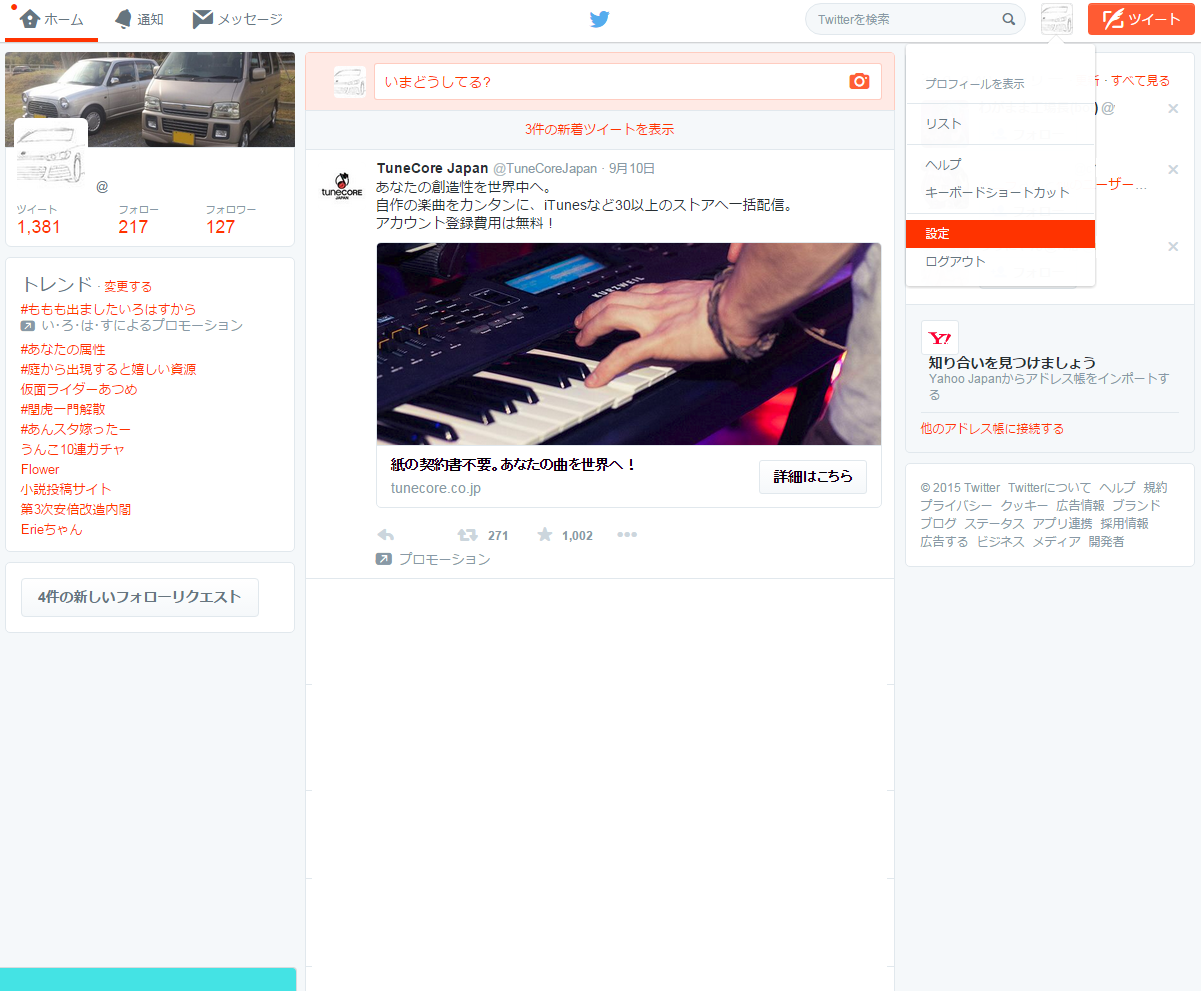
\includegraphics[width=13cm]{TwitterHome.png}
\caption{プルダウンメニューの表示}\label{pulldown}
\end{figure}

左側のメニューより「モバイル」を選択し,携帯電話番号を入力して「続ける」をクリックする.

\begin{figure}[H]
\centering
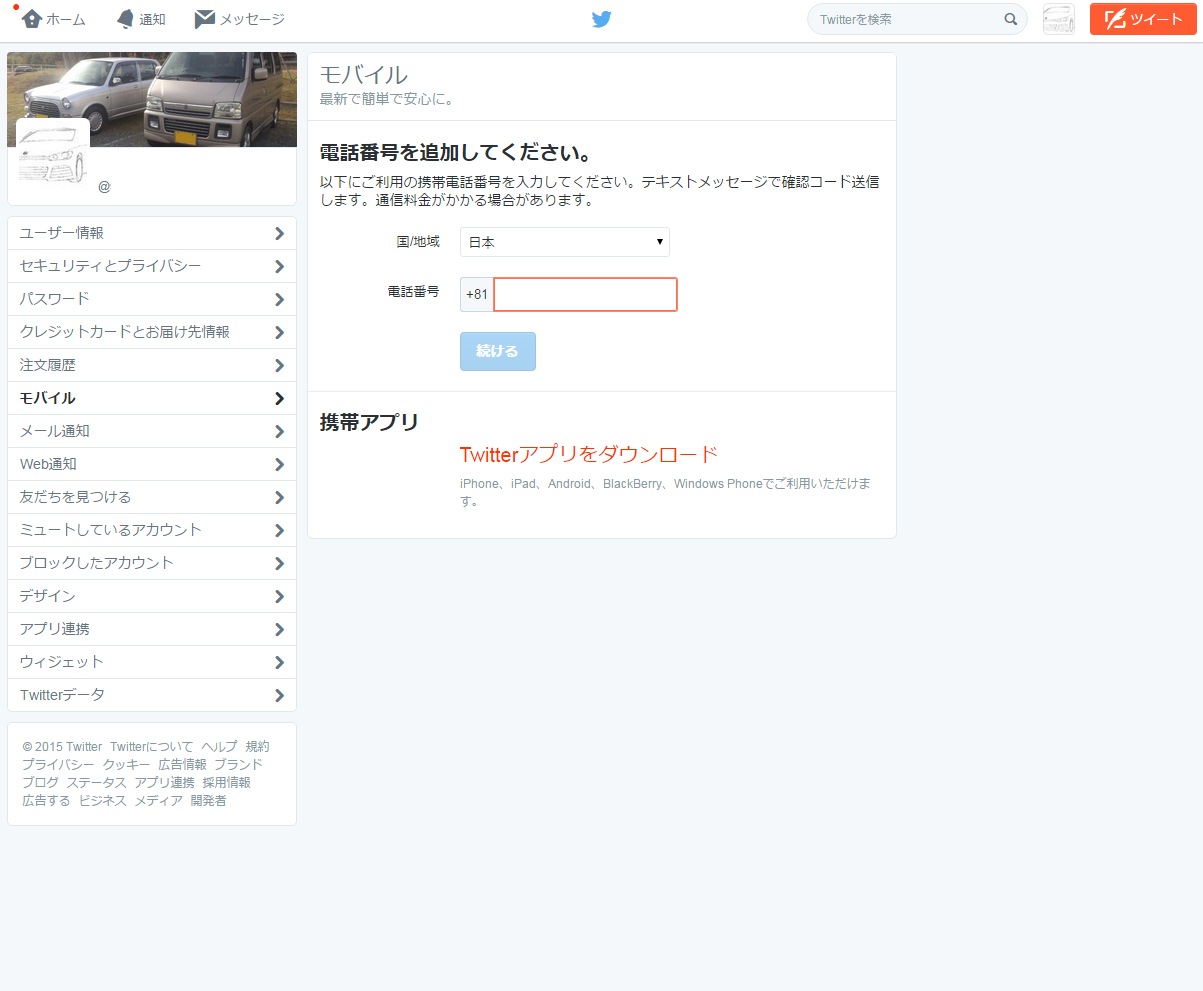
\includegraphics[width=13cm]{TwitterMobile1.png}
\caption{携帯電話番号の入力画面}\label{mobile1}
\end{figure}

入力した携帯電話番号宛に認証用コードが記載されたメッセージが届くので,その認証用コードをテキストボックス内に入力し,「携帯電話を認証する」をクリックすると「携帯電話は有効化されました.」と表示されて携帯電話の認証が完了する.

\begin{figure}[H]
\centering
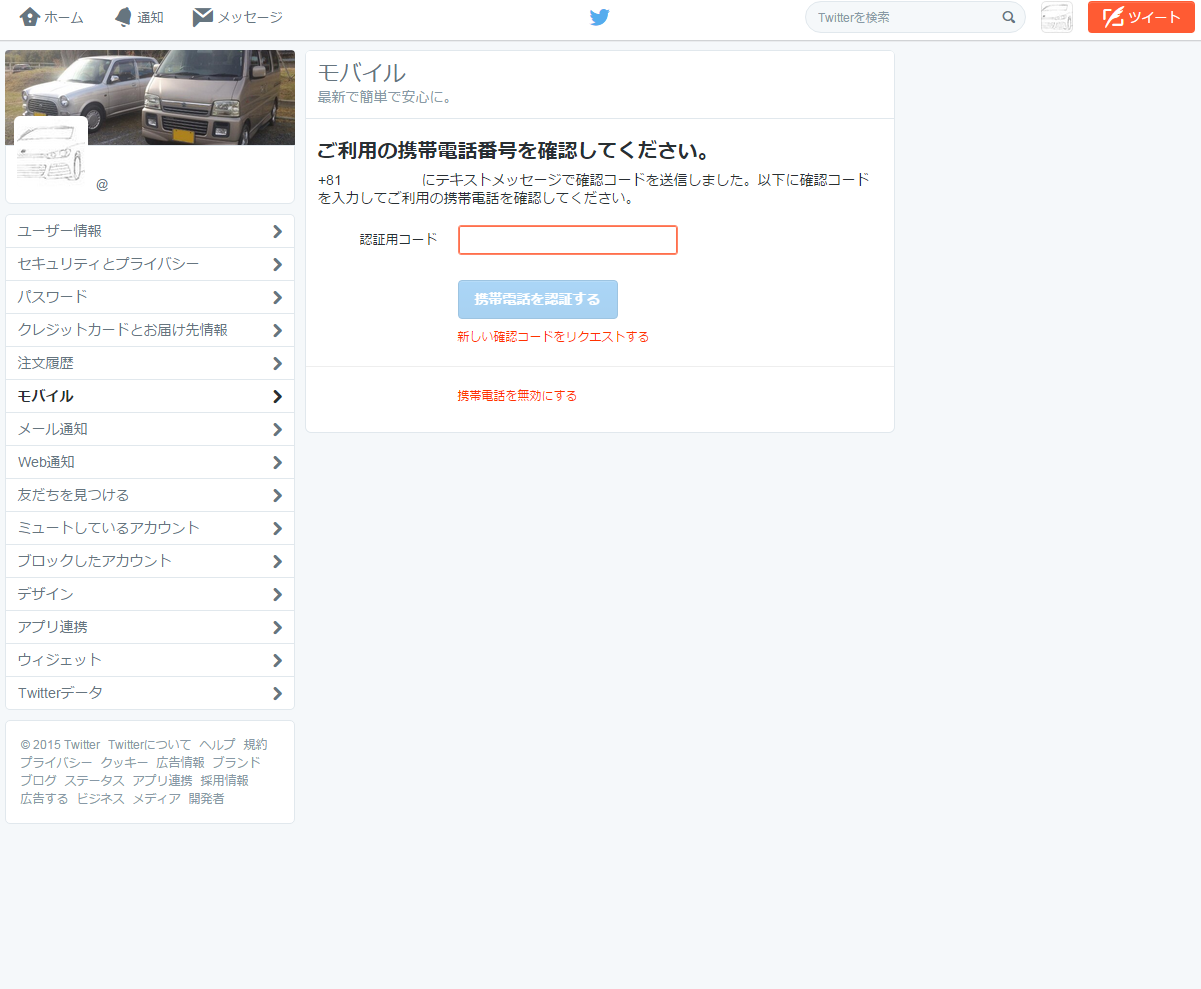
\includegraphics[width=13cm]{TwitterMobile2.png}
\caption{認証用コードの入力画面}\label{mobile2}
\end{figure}

\subsection{アプリケーションの登録}
Twitterの開発者向けページ(https://dev.twitter.com)にアクセスし,ページ下方にある「Manage Your Apps」(下図の赤枠で囲った部分)をクリックする.

\begin{figure}[H]
\centering
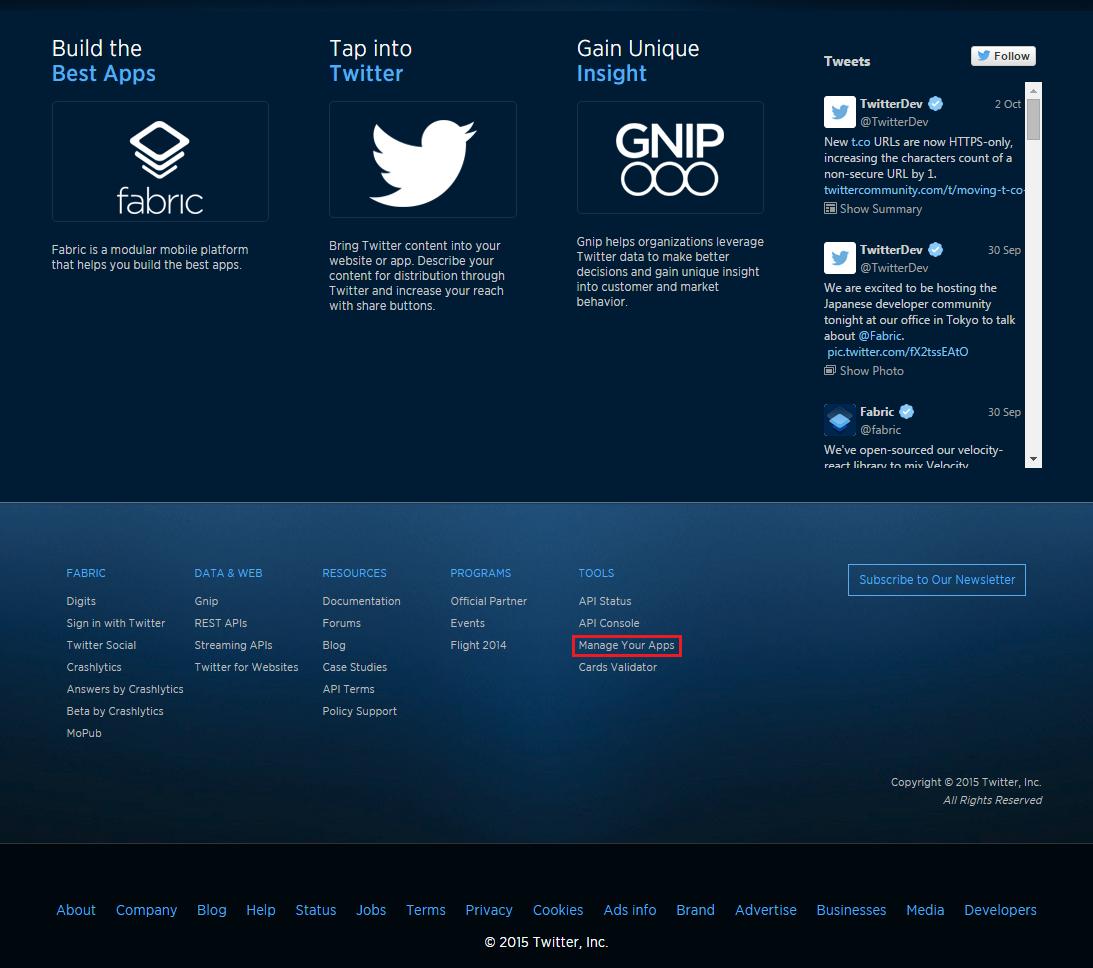
\includegraphics[width=13cm]{dev_twitter.PNG}
\caption{Twitterの開発者向けページ}\label{devTwitter}
\end{figure}
	
「You don't currently have any Twitter Apps.」と表示されるので,その下にある「Create New App」をクリックし,アプリケーション作成画面に移る.

\begin{figure}[H]
\centering
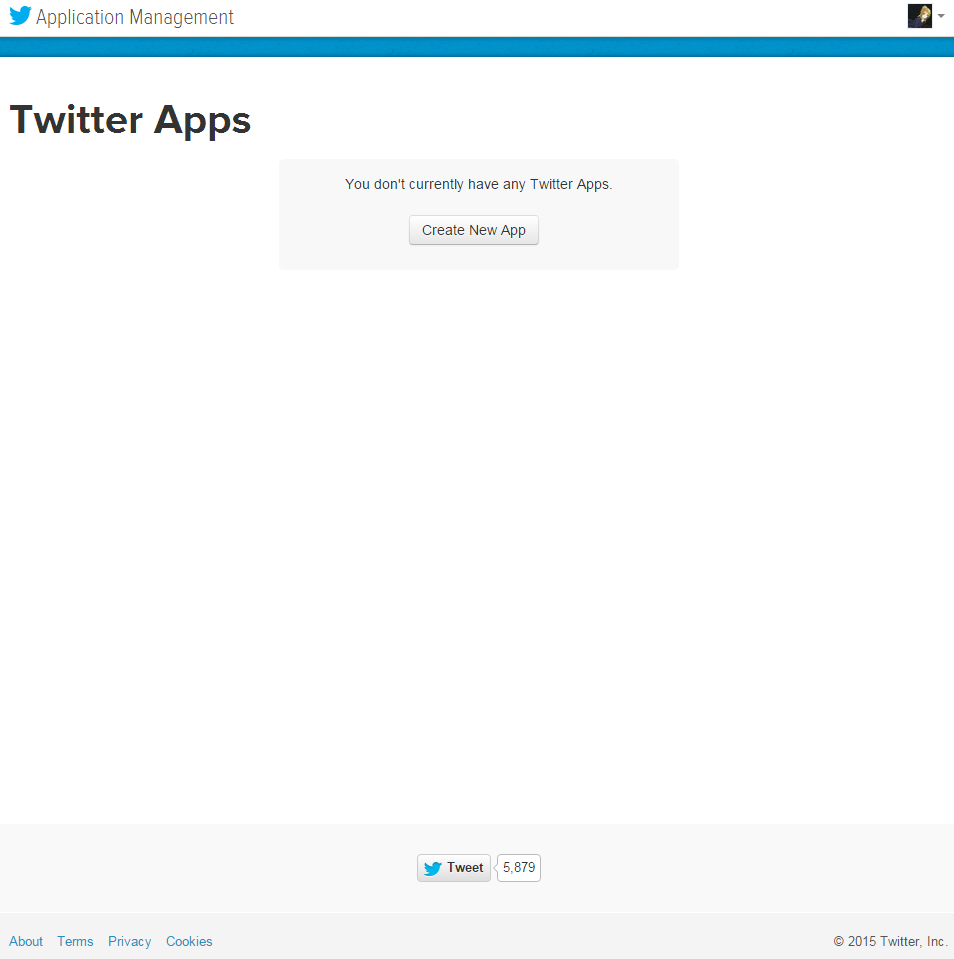
\includegraphics[width=13cm]{You_dont_currently_have_any_Twitter_Apps.PNG}
\caption{アプリケーションを作成するかどうか尋ねる画面}\label{donthaveapp}
\end{figure}

「Name(アプリケーションの名前)」,「Description(アプリケーションの説明)」,「Website(アプリケーションを動かすWebサイトのトップページのURLを本来入力しなければならないが,本研究ではそういったWebサイトを持たないため,ここでは自分のTwitterアカウントのプロフィールページのURLを記載しておく)」をそれぞれ入力する.入力を終えたら「Yes, I agree」にチェックを入れて規約に同意し,「Create your Twitter application」をクリックするとアプリケーションが作成される.%携帯の認証できないから書ききれてるかどうか怪しいけどたぶん大丈夫

\begin{figure}[H]
\centering
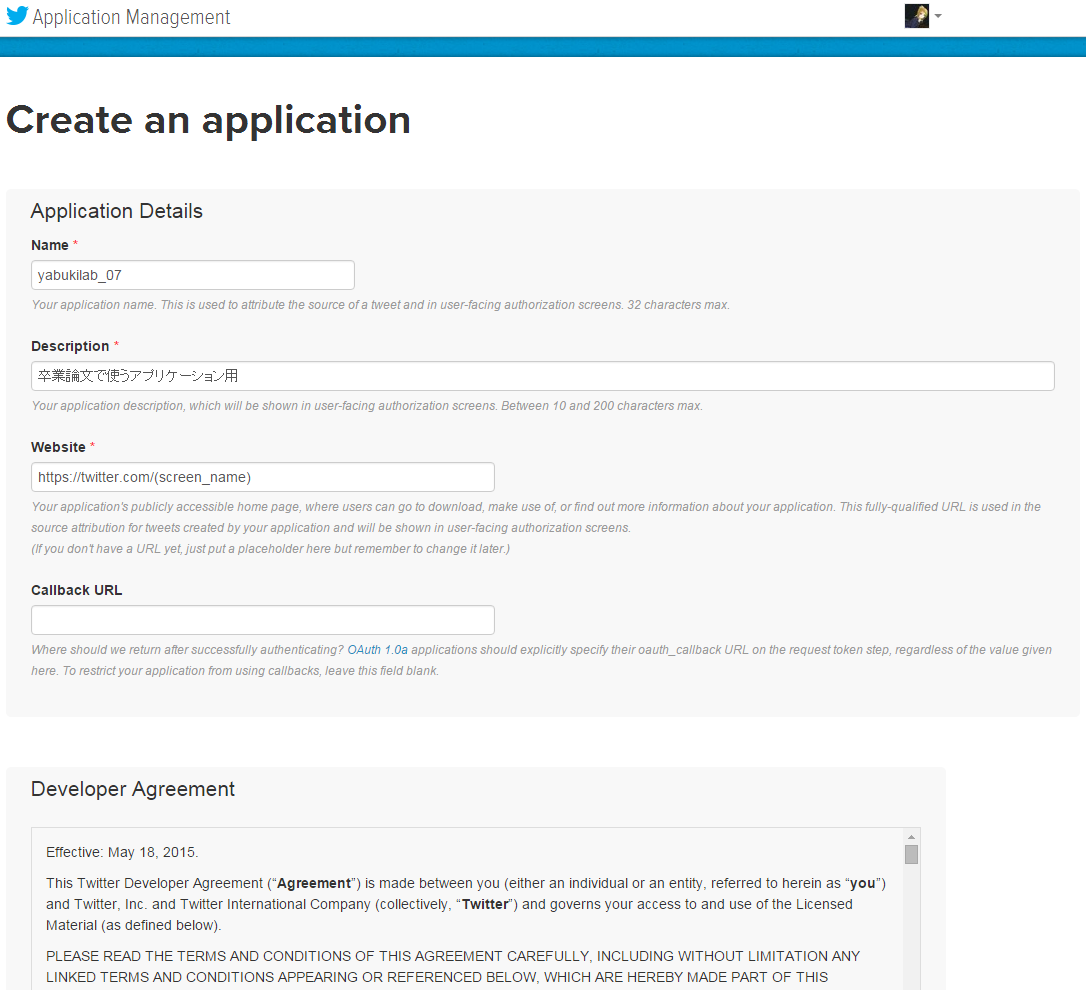
\includegraphics[width=13cm]{create_an_application.PNG}
\caption{アプリケーション作成画面}\label{createapp}
\end{figure}

これにより,後述するプログラムに必要な情報(Consumer Key,Consumer Secret,Access Token,Access Token Secret)を取得することができる.ただし,Access TokenとAccess Token Secretに関してはアカウントごとに作成する必要があるため,それらを作成するためのWebサービスを用いる.

\subsection{TwitterアカウントごとのAccess Tokenの取得}
ブラウザでhttp://getaccesstoken.herokuapp.com/にアクセスし,表示されたページの指示に従って作成したアプリケーションの設定を変更する.
	
\begin{figure}[H]
\centering
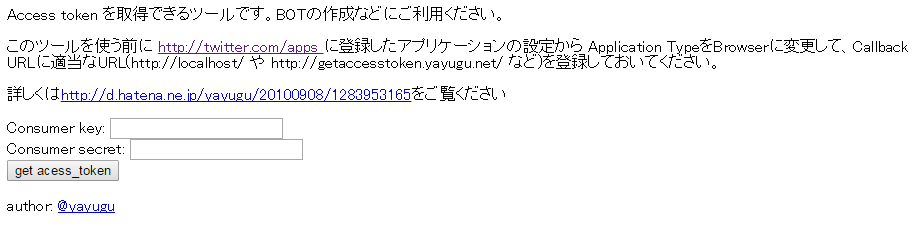
\includegraphics[width=13cm]{get_access_token.PNG}
\caption{http://getaccesstoken.herokuapp.com/の表示}\label{getaccesstoken}
\end{figure}

変更が済んだら,ブラウザであらかじめAccess TokenとAccess Token Secretを取得したいアカウントでログインし,再び上記サイトにアクセスする.「Consumer key」,「Consumer secret」に自分のアカウントのそれぞれの情報を入力し,「get acess\_token」をクリックするとAccess TokenとAccess Token Secretが表示されるため,これらをメモしておく.

\subsection{タイムラインの取得}
「端末」を起動して,下記のプログラム(stream.py)を24時間ないしそれ以上の時間実行させる(consumer\_keyとconsumer\_secretはアプリケーション作成時に取得した自分のアカウントのそれぞれの情報を,access\_tokenとaccess\_token\_secretは各々のアカウントの情報を予め入力しておく).
		
		\begin{lstlisting}[caption={}, label={}]
		# -*- coding: utf-8 -*-
 
		from tweepy.streaming import StreamListener
		from tweepy import OAuthHandler
		from tweepy import Stream
 
		consumer_key = ""
		consumer_secret = ""
 
		access_token = ""
		access_token_secret = ""
 
		class StdOutListener(StreamListener):
    			def on_data(self, data):
        			if data.startswith("{"):
            				print data
        			return True
 
    			def on_error(self, status):
        			print status
 
		if __name__ == '__main__':
    			l = StdOutListener()
    			auth = OAuthHandler(consumer_key, consumer_secret)
    			auth.set_access_token(access_token, access_token_secret)
 
    			stream = Stream(auth, l)
    			stream.userstream()
		\end{lstlisting}

ただし,長時間このプログラムを動作させていると,Tweepyのエラーによってプロセスが停止し,タイムラインの取得が途中で止まってしまうおそれがあるため,下記のスクリプトを実行してタイムラインの取得を継続できるようにする.
		
		\begin{lstlisting}[caption={}, label={}]
		#!/usr/bin/env bash
 
		while :
		do
			python stream.py >> result.txt
			sleep 240
		done
		\end{lstlisting}

\subsection{取得したタイムラインの処理}
取得したタイムラインはJSON形式で保存されており(result.txtというファイルに保存されている),この形式のままではつぶやきを閲覧したり,分析することができない.そこで下記のparse.pyを用いて必要なデータだけを,正しく読める形にして抽出する.「端末」に「python parse.py 20151023194000 20151024194000 < result.txt > result2.txt」と入力して実行すると,日本時間の2015年10月23日19時40分00秒から2015年10月24日19時40分00秒のつぶやきの本文のみが抽出され,result2.txtというファイルに保存される.
		
		\begin{lstlisting}[caption={}, label={}]
		#!/usr/bin/env python
		import sys, json, time, calendar
		#from pprint import pprint
 
		def YmdHMS(created_at):
			time_utc = time.strptime(created_at, '%a %b %d %H:%M:%S +0000 %Y')
			unix_time = calendar.timegm(time_utc)
			time_local = time.localtime(unix_time)
			return int(time.strftime("%Y%m%d%H%M%S", time_local))
 
		argv = sys.argv
		start_time = 0
		end_time = 99999999999999
		if 1 < len(argv):
			start_time = int(argv[1])
			end_time = int(argv[2])
 
		for line in sys.stdin:
			try:
				tweet = json.loads(line)
        			#pprint(tweet)
            				tweet_time = YmdHMS(tweet['created_at'])
            				if start_time <= tweet_time and tweet_time <= end_time:
                				tweet_sec = tweet_time-start_time
                				screen_name = tweet['user']['screen_name']
                				text = tweet['text'].encode('utf-8')
                				url = "https://twitter.com/#!/%s/status/%s"\
                    					% (screen_name, tweet['id_str'])
                				#print tweet_sec, url, text
                				#print text
                				t = time.strptime(str(tweet_time), "%Y%m%d%H%M%S")
                				print text
    			except StandardError:
        			pass
		\end{lstlisting}
		
\subsection{タイムラインをMeCabで分析}
上記手順で取得したタイムラインに含まれる単語を,オープンソースの形態素解析エンジンであるMeCabで抽出する.

\subsubsection{MeCabのインストール}
「端末」を開き,以下のコマンドを実行するとMeCabがインストールされる.
		
		\begin{lstlisting}[caption={}, label={}]
		sudo apt-get -y install mecab mecab-ipadic-utf8
		\end{lstlisting}

\subsubsection{分析の実行}
以下のコマンドを実行すると,各タイムライン内に出現する単語とそのTF(Term Frequency,単語の出現頻度)がMicrosoft Excel(以下,Excelと表記する)ブックファイルに書き込まれる.

		\begin{lstlisting}[caption={}, label={}]
		mecab < result2.txt | awk -F',' '{print $1}' | awk '$2=="名詞"||$2=="動詞"||$2=="形容詞"{print $1;}' | sort | uniq -c | sort -n >> result.xlsx
		\end{lstlisting}

\subsubsection{IDF, TFIDFの計算}
TFを算出しただけでは,どのタイムラインにおいても頻出するであろうありきたりな単語(「おはよう」「(~)する」など)が上位を占めてしまい,タイムラインの特徴を示しづらくなる.そこで,そういった単語の重みを軽くするためにIDF(Inverse Document Frequency,逆文書頻度)を算出する.TFとIDFを掛けあわせたTFIDFの数値が高い単語が,よりタイムラインごとの特徴といえる語になる.IDFは,「Inverse」の名が示すように対数をとった計算であり,次式のように示される.

\[
	\log \frac{\textrm{タイムラインの総数}}{\textrm{その単語が出現するタイムラインの数}}
\]

Excelでこの式の計算をする際は,「=LOG(タイムラインの総数/その単語が出現するタイムラインの数)」のように入力する.また,TFIDFの式は「=TF*IDF」のように入力する.

\chapter{結果}

\section{本章の構成}
本章では,自分と5人の協力者それぞれのTwitterでの利用スタイルや関心事項と,TFIDFの値が高い単語上位20個のワードクラウドやTFIDF値とを比較する.

\section{ワードクラウドとは}
SNSをはじめとするWebサイトなどにある文章から,単語の出現頻度や品詞を分析した結果を大きさや色の違いを用いてその単語を表示し,それらを集めたもの.

\section{ワードクラウドの見方}
TFIDFの値が高い単語はより大きく表示され,そのタイムラインを特徴づけているといえる.色は品詞を表しており,青は名詞,緑は形容詞,橙は動詞である.

\section{自分の場合}

\subsection{利用スタイル}
長時間にわたってタイムラインを閲覧することと,リツイートを行うことが多い.それらと比べると,自分の言葉でつぶやく回数は少ない.

\subsection{関心事項}
\begin{itemize}
	\item バーチャルアイドル「初音ミク」に関する話題やイラスト,音楽など
	\item スポーツカーに乗る人のつぶやきやアップロードする写真
	\item PCやスマートフォン,タブレット端末など,ガジェットに関する最新の情報
	\item 世界で起こる様々なニュース
\end{itemize}

\subsection{結果}

\begin{figure}[H]
\centering
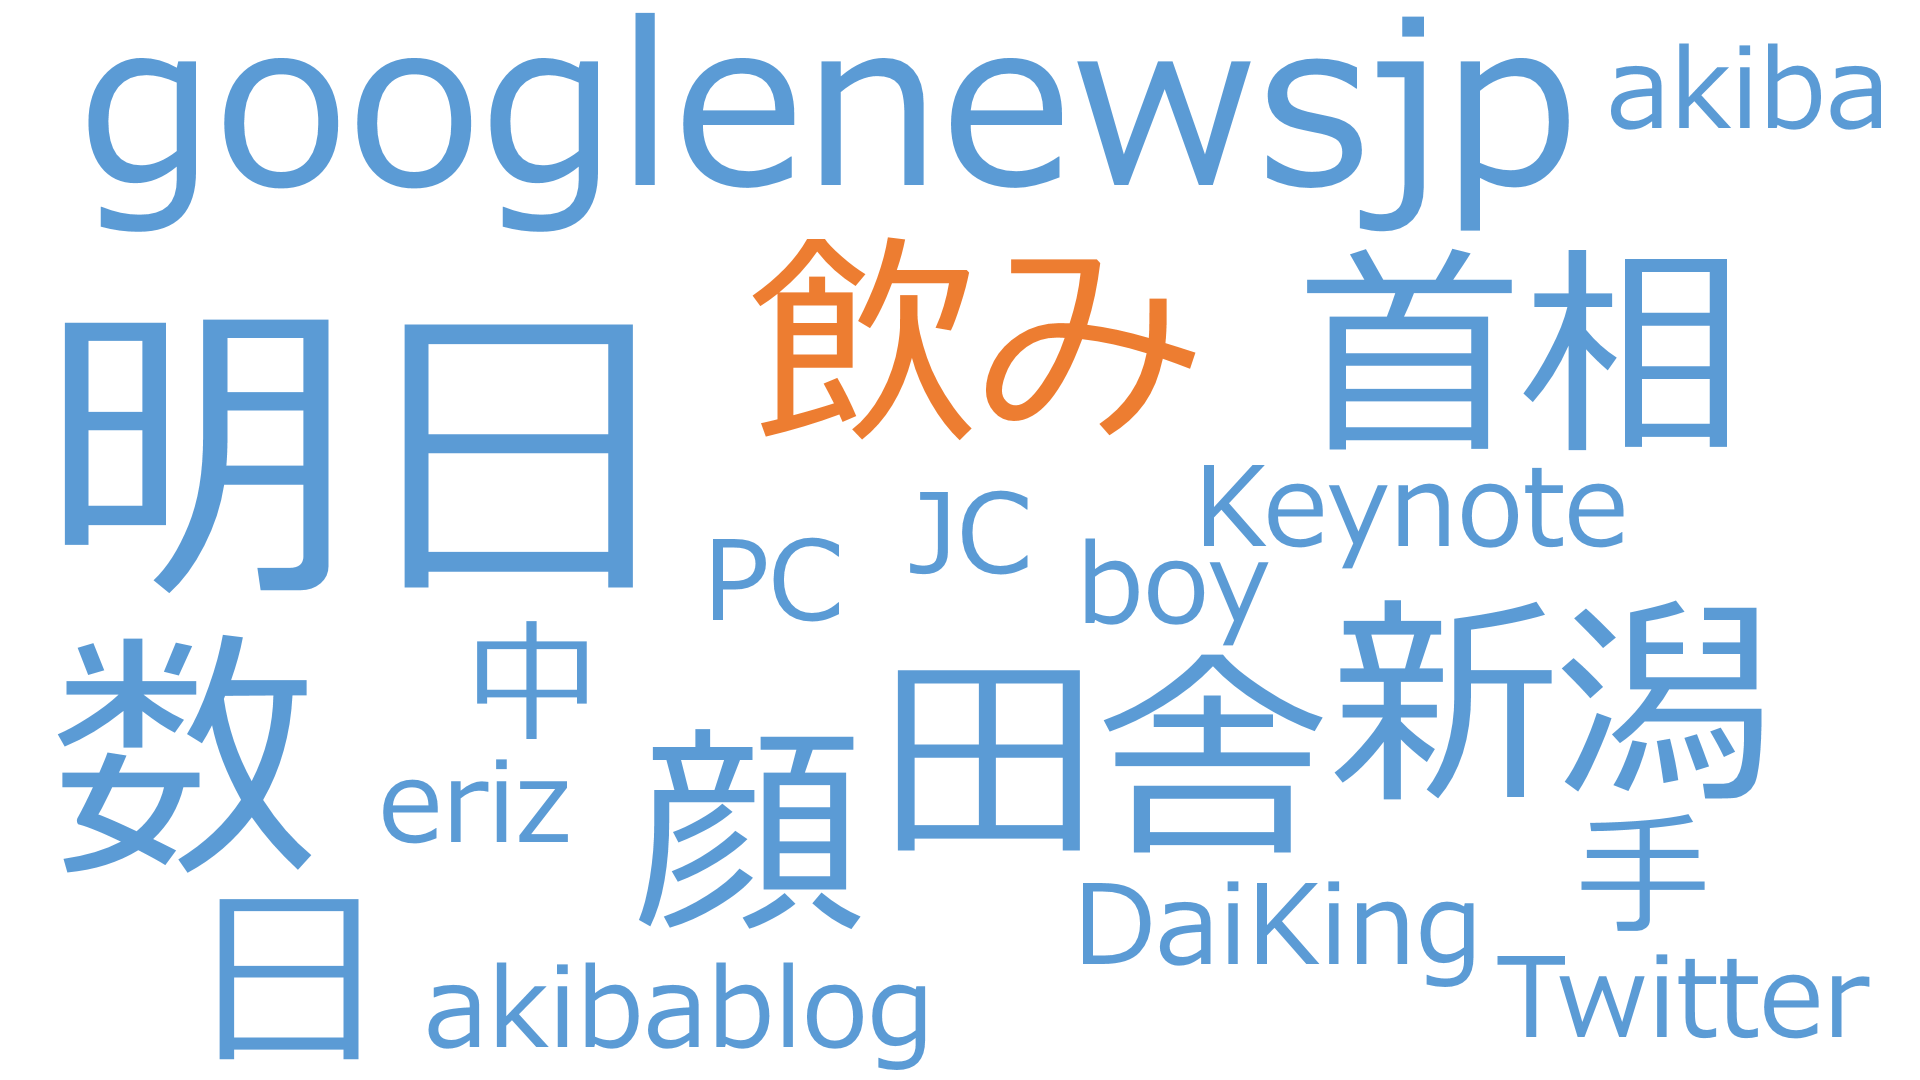
\includegraphics[width=13cm]{yoshino_cloud.png}
\caption{自分のワードクラウド}\label{yoshinocloud}
\end{figure}

\begin{table}[H]
	\centering
	\caption{自分のTFIDF}
	\begin{tabular}{l|c|c|c|c}
		単語 & TF & 出現タイムライン数 & IDF & TFIDF \\ \hline
		明日 & 3 & 1 & 0.77815125 & 2.334453751 \\
		数 & 4 & 2 & 0.477121255 & 1.908485019 \\
		googlenewsjp & 2 & 1 & 0.77815125 & 1.556302501 \\
		飲み & 2 & 1 & 0.77815125 & 1.556302501 \\
		顔 & 2 & 1 & 0.77815125 & 1.556302501 \\
		首相 & 2 & 1 & 0.77815125 & 1.556302501 \\
		新潟 & 2 & 1 & 0.77815125 & 1.556302501 \\
		田舎 & 2 & 1 & 0.77815125 & 1.556302501 \\
		日 & 3 & 2 & 0.477121255 & 1.431363764 \\
		手 & 2 & 2 & 0.477121255 & 0.954242509 \\
		中 & 2 & 2 & 0.477121255 & 0.954242509 \\
		DaiKing & 1 & 1 & 0.77815125 & 0.77815125 \\
		JC & 1 & 1 & 0.77815125 & 0.77815125 \\
		Keynote & 1 & 1 & 0.77815125 & 0.77815125 \\
		PC & 1 & 1 & 0.77815125 & 0.77815125 \\
		Twitter & 1 & 1 & 0.77815125 & 0.77815125 \\
		akiba & 1 & 1 & 0.77815125 & 0.77815125 \\
		akibablog & 1 & 1 & 0.77815125 & 0.77815125 \\
		boy & 1 & 1 & 0.77815125 & 0.77815125 \\
		eriz & 1 & 1 & 0.77815125 & 0.77815125
	\end{tabular}
\end{table}

\section{協力者Aの場合}

\subsection{利用スタイル}
タイムラインを閲覧するのみで,自分はつぶやかない

\subsection{関心事項}
\begin{itemize}
	\item 声優のつぶやき
	\item マンガ家のつぶやき
	\item コスプレの写真
	\item キャラクターのセリフを定期的につぶやくボット
\end{itemize}

\subsection{結果}

\begin{figure}[H]
\centering
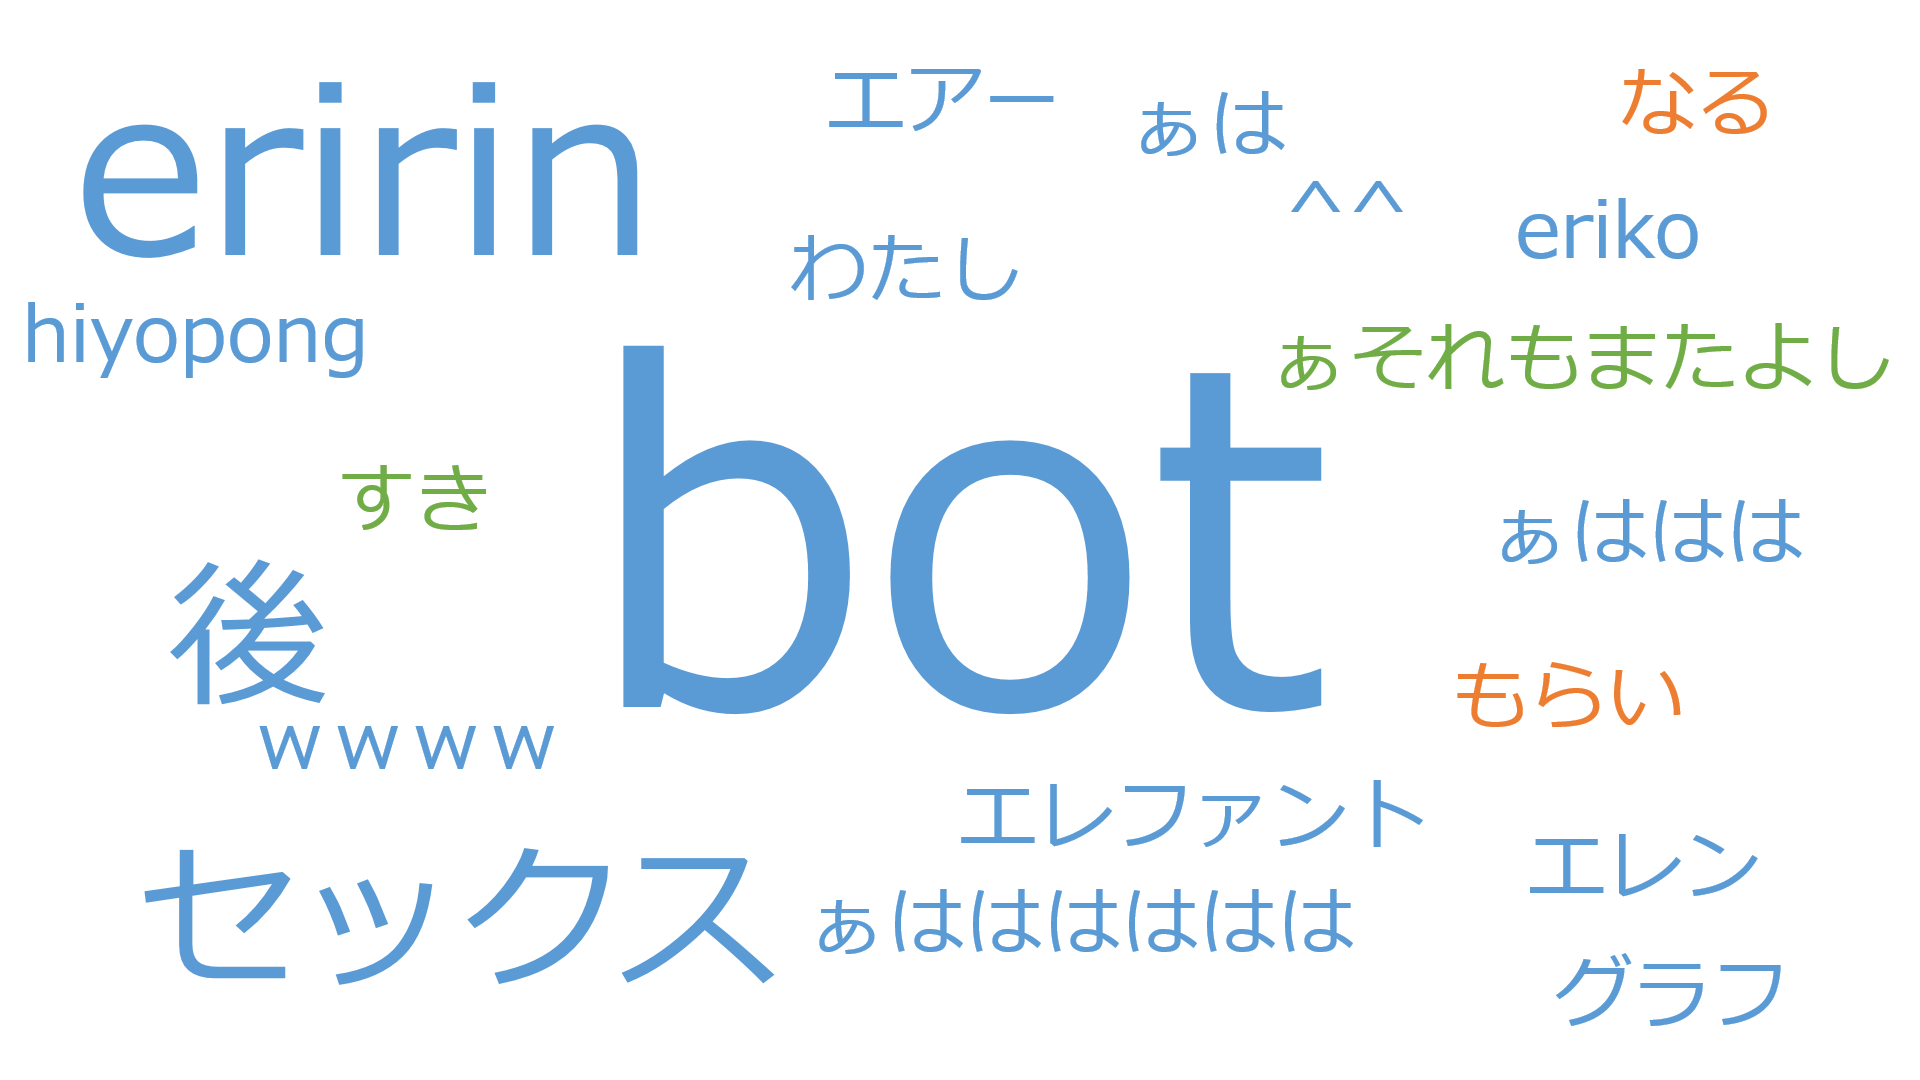
\includegraphics[width=13cm]{izumi_cloud.png}
\caption{協力者Aのワードクラウド}\label{izumicloud}
\end{figure}

\begin{table}[H]
	\centering
	\caption{協力者AのTFIDF}
	\begin{tabular}{l|c|c|c|c}
		単語 & TF & 出現タイムライン数 & IDF & TFIDF \\ \hline
		bot & 6 & 1 & 0.77815125 & 4.668907502 \\
		eririn & 3 & 1 & 0.77815125 & 2.334453751 \\
		セックス & 2 & 1 & 0.77815125 & 1.556302501 \\
		後 & 2 & 1 & 0.77815125 & 1.556302501 \\
		\verb|^|\verb|^| & 1 & 1 & 0.77815125 & 0.77815125 \\
		eriko & 1 & 1 & 0.77815125 & 0.77815125 \\
		hiyopong & 1 & 1 & 0.77815125 & 0.77815125 \\
		wwww & 1 & 1 & 0.77815125 & 0.77815125 \\
		ぁそれもまたよし & 1 & 1 & 0.77815125 & 0.77815125 \\
		ぁは & 1 & 1 & 0.77815125 & 0.77815125 \\
		ぁははは & 1 & 1 & 0.77815125 & 0.77815125 \\
		ぁはははははは & 1 & 1 & 0.77815125 & 0.77815125 \\
		すき & 1 & 1 & 0.77815125 & 0.77815125 \\
		なる & 1 & 1 & 0.77815125 & 0.77815125 \\
		もらい & 1 & 1 & 0.77815125 & 0.77815125 \\
		わたし & 1 & 1 & 0.77815125 & 0.77815125 \\
		エアー & 1 & 1 & 0.77815125 & 0.77815125 \\
		エレファント & 1 & 1 & 0.77815125 & 0.77815125 \\
		エレン & 1 & 1 & 0.77815125 & 0.77815125 \\
		グラフ & 1 & 1 & 0.77815125 & 0.77815125
	\end{tabular}
\end{table}

\section{協力者Bの場合}

\subsection{利用スタイル}
タイムラインの閲覧

\subsection{関心事項}
公式アカウント(ゲーム「アイドルマスター」公式アカウント等)のつぶやき

\subsection{結果}

\begin{figure}[H]
\centering
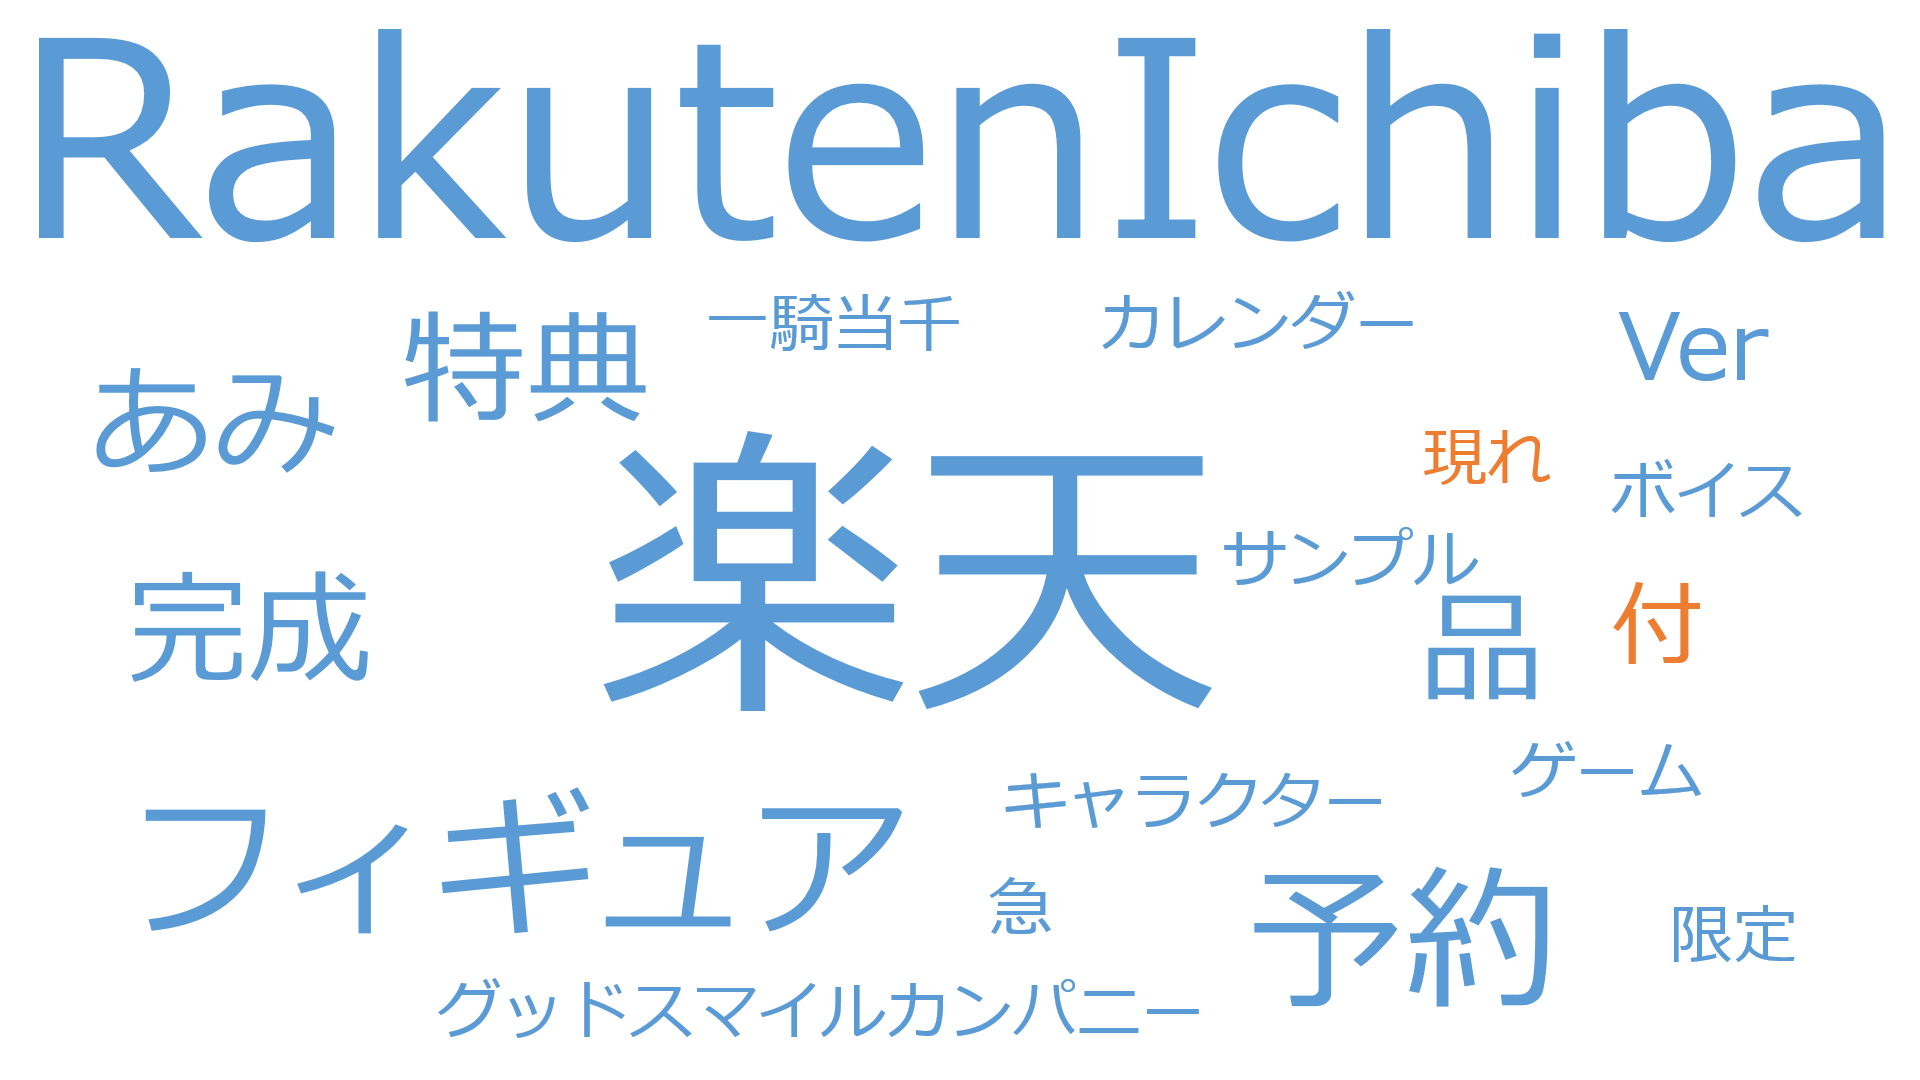
\includegraphics[width=13cm]{itakura_cloud.png}
\caption{協力者Bのワードクラウド}\label{itakuracloud}
\end{figure}

\begin{table}[H]
	\centering
	\caption{協力者BのTFIDF}
	\begin{tabular}{l|c|c|c|c}
		単語 & TF & 出現タイムライン数 & IDF & TFIDF \\ \hline
		楽天 & 10 & 1 & 0.77815125 & 7.781512504 \\
		RakutenIchiba & 9 & 1 & 0.77815125 & 7.003361253 \\
		フィギュア & 5 & 1 & 0.77815125 & 3.890756252 \\
		予約 & 5 & 1 & 0.77815125 & 3.890756252 \\
		あみ & 4 & 1 & 0.77815125 & 3.112605002 \\
		完成 & 4 & 1 & 0.77815125 & 3.112605002 \\
		特典 & 4 & 1 & 0.77815125 & 3.112605002 \\
		品 & 4 & 1 & 0.77815125 & 3.112605002 \\
		Ver & 3 & 1 & 0.77815125 & 2.334453751 \\
		付 & 3 & 1 & 0.77815125 & 2.334453751 \\
		カレンダー & 2 & 1 & 0.77815125 & 1.556302501 \\
		キャラクター & 2 & 1 & 0.77815125 & 1.556302501 \\
		グッドスマイルカンパニー & 2 & 1 & 0.77815125 & 1.556302501 \\
		ゲーム & 2 & 1 & 0.77815125 & 1.556302501 \\
		サンプル & 2 & 1 & 0.77815125 & 1.556302501 \\
		ボイス & 2 & 1 & 0.77815125 & 1.556302501 \\
		一騎当千 & 2 & 1 & 0.77815125 & 1.556302501 \\
		急 & 2 & 1 & 0.77815125 & 1.556302501 \\
		現れ & 2 & 1 & 0.77815125 & 1.556302501 \\
		限定 & 2 & 1 & 0.77815125 & 1.556302501
	\end{tabular}
\end{table}

\section{協力者Cの場合}

\subsection{利用スタイル}
自分の思っていることや,面白い出来事をつぶやきにして発信する

\subsection{関心事項}
自分のつぶやきが共感を得られているかどうか

\subsection{結果}

\begin{figure}[H]
\centering
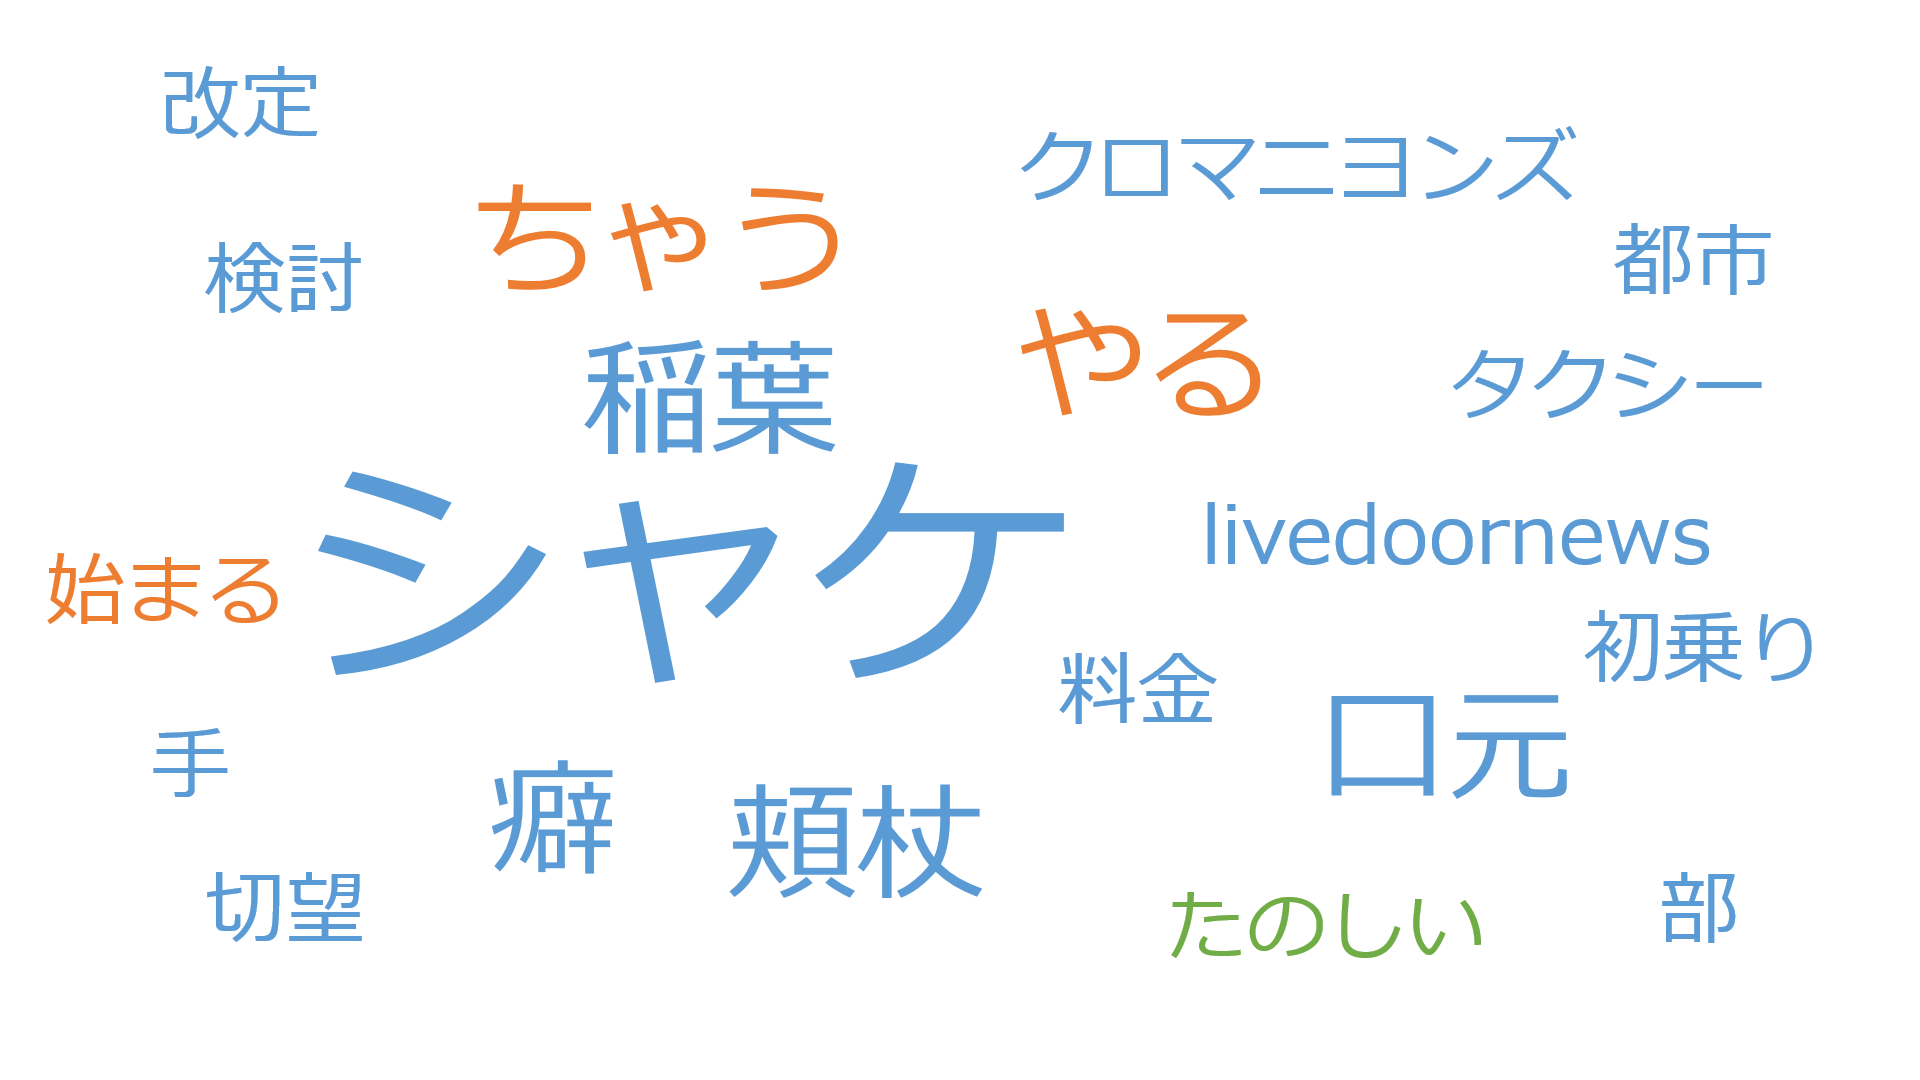
\includegraphics[width=13cm]{kawate_cloud.png}
\caption{協力者Cのワードクラウド}\label{kawatecloud}
\end{figure}

\begin{table}[H]
	\centering
	\caption{協力者CのTFIDF}
	\begin{tabular}{l|c|c|c|c}
		単語 & TF & 出現タイムライン数 & IDF & TFIDF \\ \hline
		シャケ & 2 & 1 & 0.77815125 & 1.556302501 \\
		ちゃう & 1 & 1 & 0.77815125 & 0.77815125 \\
		やる & 1 & 1 & 0.77815125 & 0.77815125 \\
		稲葉 & 1 & 1 & 0.77815125 & 0.77815125 \\
		口元 & 1 & 1 & 0.77815125 & 0.77815125 \\
		癖 & 1 & 1 & 0.77815125 & 0.77815125 \\
		頬杖 & 1 & 1 & 0.77815125 & 0.77815125 \\
		livedoornews & 1 & 2 & 0.477121255 & 0.477121255 \\
		たのしい & 1 & 2 & 0.477121255 & 0.477121255 \\
		クロマニヨンズ & 1 & 2 & 0.477121255 & 0.477121255 \\
		タクシー & 1 & 2 & 0.477121255 & 0.477121255 \\
		改定 & 1 & 2 & 0.477121255 & 0.477121255 \\
		検討 & 1 & 2 & 0.477121255 & 0.477121255 \\
		始まる & 1 & 2 & 0.477121255 & 0.477121255 \\
		手 & 1 & 2 & 0.477121255 & 0.477121255 \\
		初乗り & 1 & 2 & 0.477121255 & 0.477121255 \\
		切望 & 1 & 2 & 0.477121255 & 0.477121255 \\
		都市 & 1 & 2 & 0.477121255 & 0.477121255 \\
		部 & 1 & 2 & 0.477121255 & 0.477121255 \\
		料金 & 1 & 2 & 0.477121255 & 0.477121255
	\end{tabular}
\end{table}

\section{協力者Dの場合}

\subsection{利用スタイル}
\begin{itemize}
	\item 趣味に関する情報収集
	\item フォロワーとの会話
\end{itemize}

\subsection{関心事項}
\begin{itemize}
	\item ゲームに関するつぶやき(ブラウザゲーム「艦隊これくしょん」等)
	\item イラスト
\end{itemize}

\subsection{結果}

\begin{figure}[H]
\centering
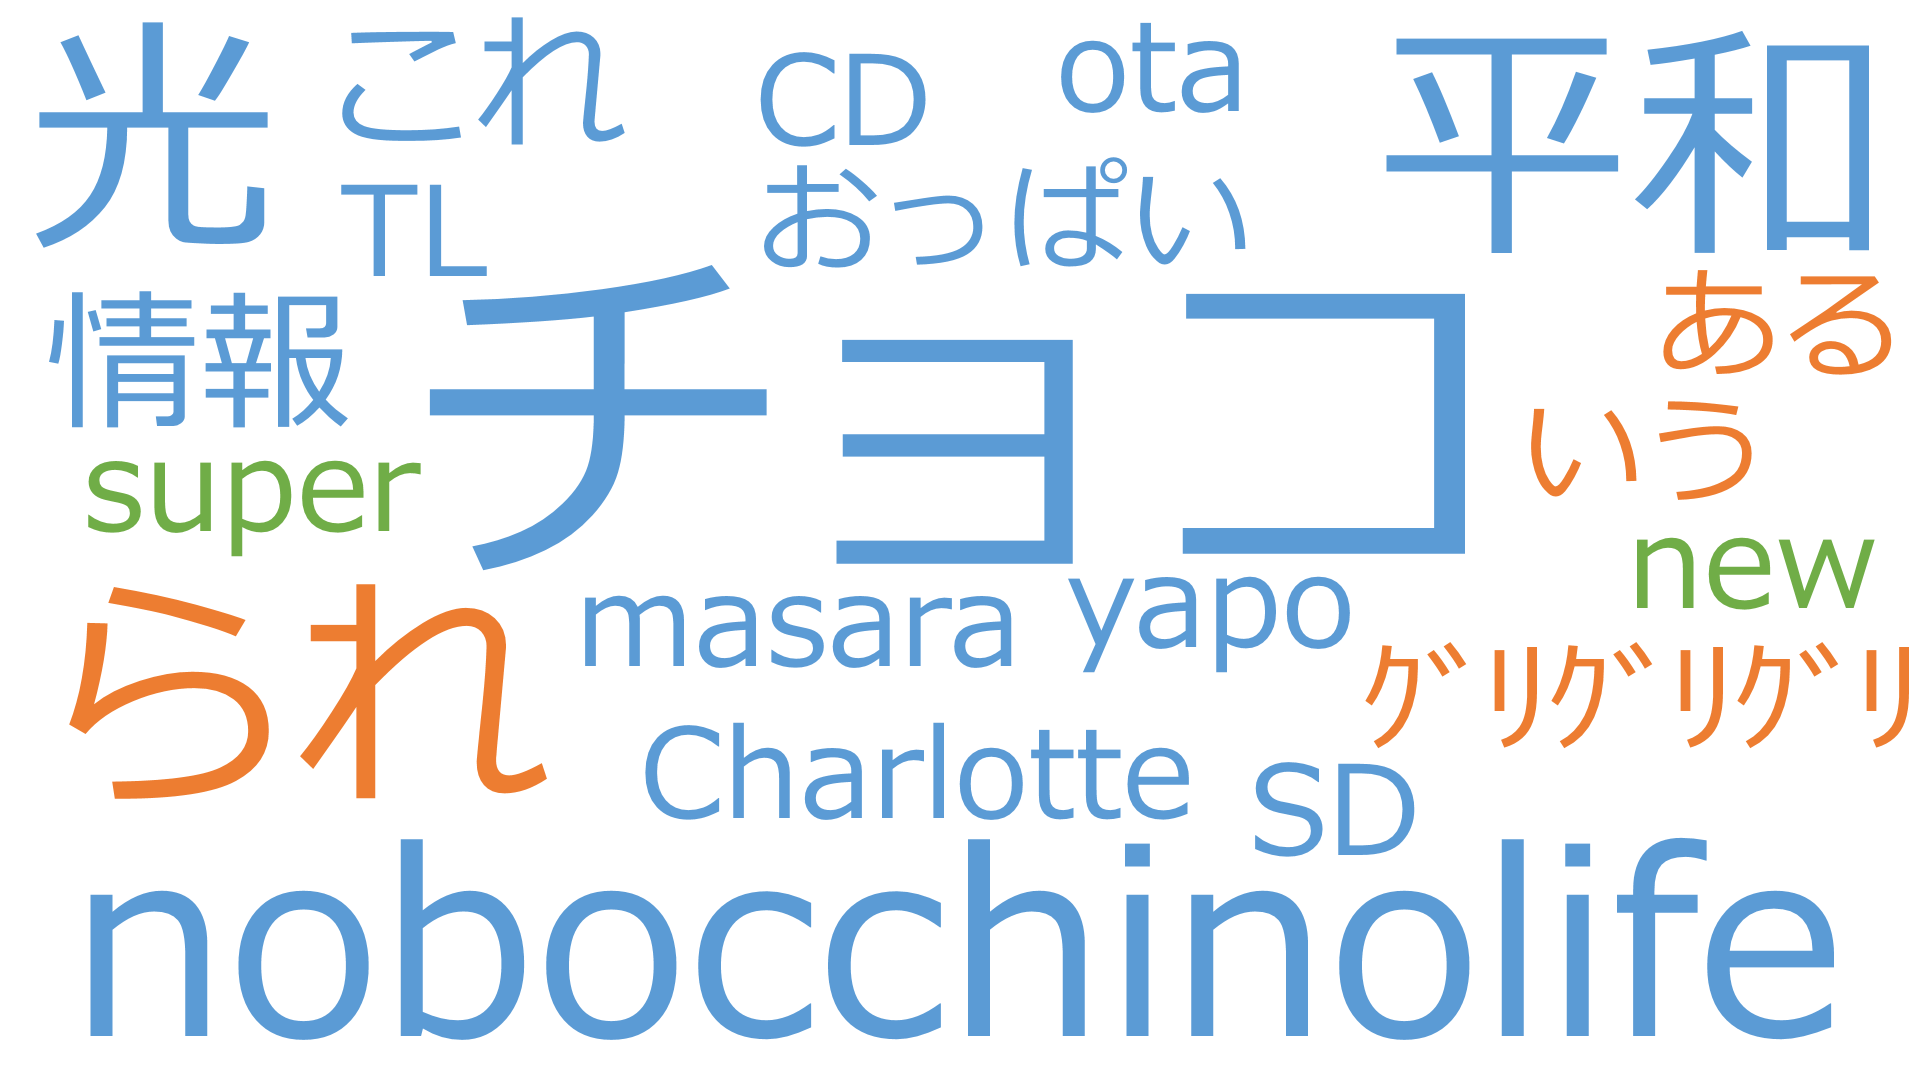
\includegraphics[width=13cm]{shimada_cloud.png}
\caption{協力者Dのワードクラウド}\label{shimadacloud}
\end{figure}

\begin{table}[H]
	\centering
	\caption{協力者DのTFIDF}
	\begin{tabular}{l|c|c|c|c}
		単語 & TF & 出現タイムライン数 & IDF & TFIDF \\ \hline
		チョコ & 3 & 1 & 0.77815125 & 2.334453751 \\
		nobocchinolife & 2 & 1 & 0.77815125 & 1.556302501 \\
		られ & 2 & 1 & 0.77815125 & 1.556302501 \\
		光 & 2 & 1 & 0.77815125 & 1.556302501 \\
		平和 & 2 & 1 & 0.77815125 & 1.556302501 \\
		これ & 2 & 2 & 0.477121255 & 0.954242509 \\
		情報 & 2 & 2 & 0.477121255 & 0.954242509 \\
		CD & 1 & 1 & 0.77815125 & 0.77815125 \\
		Charlotte & 1 & 1 & 0.77815125 & 0.77815125 \\
		SD & 1 & 1 & 0.77815125 & 0.77815125 \\
		TL & 1 & 1 & 0.77815125 & 0.77815125 \\
		masara & 1 & 1 & 0.77815125 & 0.77815125 \\
		new & 1 & 1 & 0.77815125 & 0.77815125 \\
		ota & 1 & 1 & 0.77815125 & 0.77815125 \\
		super & 1 & 1 & 0.77815125 & 0.77815125 \\
		yapo & 1 & 1 & 0.77815125 & 0.77815125 \\
		グリグリグリ & 1 & 1 & 0.77815125 & 0.77815125 \\
		ある & 1 & 1 & 0.77815125 & 0.77815125 \\
		いう & 1 & 1 & 0.77815125 & 0.77815125 \\
		おっぱい & 1 & 1 & 0.77815125 & 0.77815125
	\end{tabular}
\end{table}

\section{協力者Eの場合}

\subsection{利用スタイル}
\begin{itemize}
	\item タイムラインの閲覧
	\item 画像の投稿
\end{itemize}

\subsection{関心事項}
\begin{itemize}
	\item ゲーム「アイドルマスター」
	\item 飯テロ画像(※飯テロ:深夜の時間帯に美味しそうな食べ物の写真を投稿し,それを見た者の空腹感を誘発する行為)
\end{itemize}

\subsection{結果}

\begin{figure}[H]
\centering
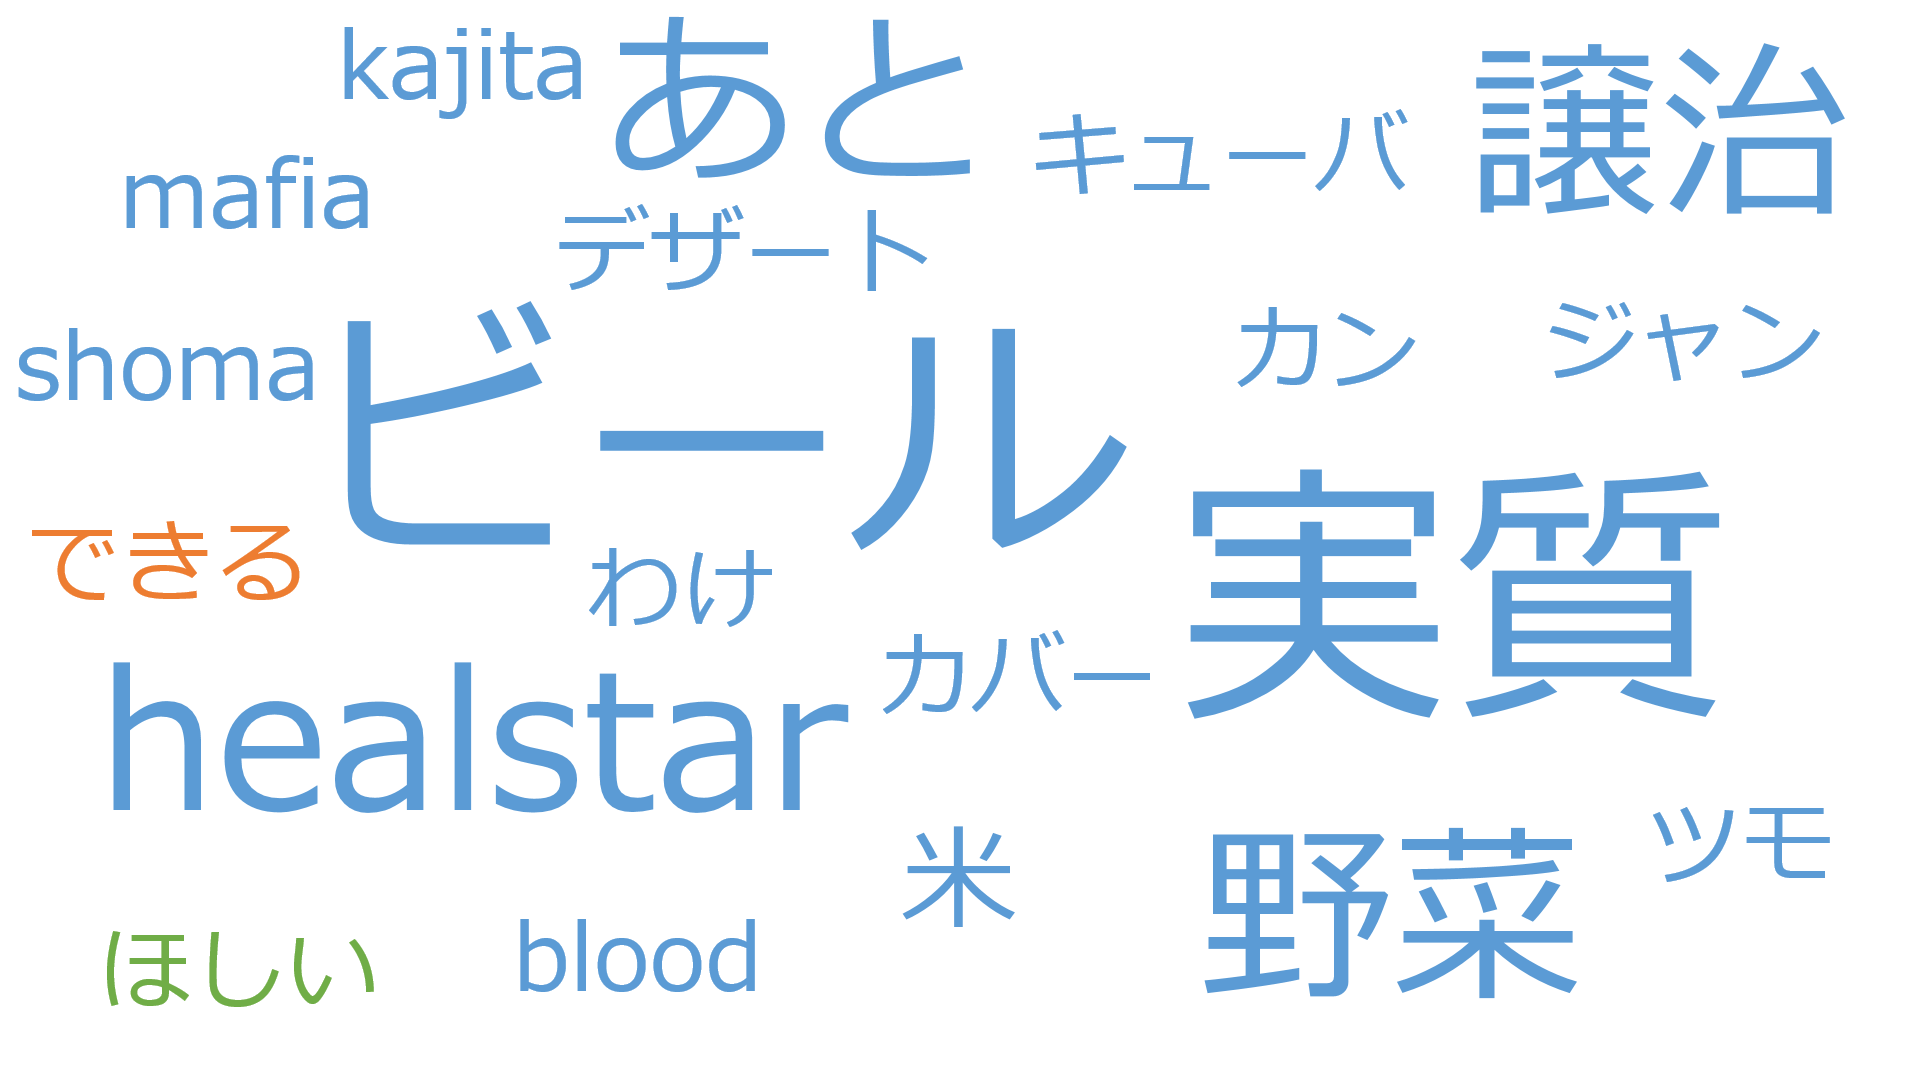
\includegraphics[width=13cm]{shimomura_cloud.png}
\caption{協力者Eのワードクラウド}\label{shimomuracloud}
\end{figure}

\begin{table}[H]
	\centering
	\caption{協力者EのTFIDF}
	\begin{tabular}{l|c|c|c|c}
		単語 & TF & 出現タイムライン数 & IDF & TFIDF \\ \hline
		ビール & 3 & 1 & 0.77815125 & 2.334453751 \\
		実質 & 3 & 1 & 0.77815125 & 2.334453751 \\
		healstar & 2 & 1 & 0.77815125 & 1.556302501 \\
		あと & 2 & 1 & 0.77815125 & 1.556302501 \\
		譲治 & 2 & 1 & 0.77815125 & 1.556302501 \\
		野菜 & 2 & 1 & 0.77815125 & 1.556302501 \\
		米 & 2 & 2 & 0.477121255 & 0.954242509 \\
		blood & 1 & 1 & 0.77815125 & 0.77815125 \\
		kajita & 1 & 1 & 0.77815125 & 0.77815125 \\
		mafia & 1 & 1 & 0.77815125 & 0.77815125 \\
		shoma & 1 & 1 & 0.77815125 & 0.77815125 \\
		できる & 1 & 1 & 0.77815125 & 0.77815125 \\
		ほしい & 1 & 1 & 0.77815125 & 0.77815125 \\
		わけ & 1 & 1 & 0.77815125 & 0.77815125 \\
		カバー & 1 & 1 & 0.77815125 & 0.77815125 \\
		カン & 1 & 1 & 0.77815125 & 0.77815125 \\
		キューバ & 1 & 1 & 0.77815125 & 0.77815125 \\
		ジャン & 1 & 1 & 0.77815125 & 0.77815125 \\
		ツモ & 1 & 1 & 0.77815125 & 0.77815125 \\
		デザート & 1 & 1 & 0.77815125 & 0.77815125
	\end{tabular}
\end{table}

\chapter{考察}

\section{自分の結果に対する考察}
関心事項として挙げた「世界で起こる様々なニュース」に関連してか,「googlenewsjp」や,「首相」が上位に入った.また,PCへの興味に関連したと思われる「Keynote(Mac,iOS向けのプレゼンテーションソフトウェア)」「PC」も上位20個のうちに入った.

\section{協力者Aの結果に対する考察}
タイムラインの取得を行う前のヒアリングで「ボットのアカウントをフォローしている」と協力者Aが話していたとおりの結果となったのか,「bot」という単語が突出して大きな値になった.
%「eririn」「eriko」とは?「hiyopong」はひよっちのbotと思われる

\section{協力者Bの結果に対する考察}
「楽天」「RakutenIchiba」の値が高かった理由として,楽天市場の商品詳細ページに設置されている「ツイート」ボタンを押すことにより,商品の詳細がTwitter上に共有され,そのつぶやきの中に「楽天」「RakutenIchiba」が入っているものと考えられる.
協力者Bが関心事項として挙げた「アイドルマスター」はゲームやCDの媒体を始めとして,様々なグッズが商品化されている.「フィギュア」「予約」「特典」「Ver」「カレンダー」「キャラクター」「グッドスマイルカンパニー(フィギュア・玩具を製造・販売するメーカー)」の単語はすべて,アイドルマスターに関連した単語と考えられる.

\section{協力者Cの結果に対する考察}
事前のヒアリングで協力者Cが回答した「自分の思っていることや,面白い出来事をつぶやきにして発信する」という利用スタイルに関連したものと思われる「たのしい」「livedoornews」が上位に入った.ここで「livedoornews」を挙げた理由として,ライブドアニュース上にある面白い記事をツイート,またはリツイートした(された)可能性が考えられる.

\section{協力者Dの結果に対する考察}
「情報」「CD」「Charlotte(アニメ作品のタイトル)」が上位に入った理由として,協力者Dが挙げた利用スタイルや関心事項に関連するものと考えられる.また,「られ」という他動詞や,「これ」という指示語が上位に入ったのは,利用スタイルのひとつであるフォロワーとの会話を盛んに行った結果として表れたものと考えられる.

\section{協力者Eの結果に対する考察}
事前のヒアリングで協力者Eが話した「飯テロ画像をリツイートする」という発言に関連したものと思われる,食べ物や飲み物の単語が多く現れる結果となった.

\chapter{結論}
本研究の対象となったユーザひとりひとりへのヒアリングの結果と,各タイムラインを特徴づける単語にいくつかの関連性を見出すことができた.これにより,本研究の手法を用いてTwitterユーザが持つ顕在的なニーズを読み取ることは,十分に可能といえる.

逆に,ヒアリングした内容との結びつきがない単語に関しては,断片的なものの集まりであることが多く,潜在的なニーズを示すには難しい結果となった.この点に関しては研究の手法に改善の余地があると考える.

\bibliographystyle{junsrt}
\bibliography{biblio}%「biblio.bib」というファイルが必要.

\end{document}